\documentclass[a4paper]{cernatsnote}
\usepackage[utf8]{inputenc}

\usepackage{subcaption}
\usepackage{graphicx}
\usepackage{longtable}
\usepackage{booktabs}
\usepackage{float}

\title{Injection optics commissioning in 2021 and 2022}
\documentlabel{CERN-ACC-NOTE-2022-YYYY}
\keywords{optics, LHC, beam-test}

\author{ T.~Persson, J.~Dilly, E.~Fol, H.~Garc\'ia Morales, M.~Hofer,
 J.~Keintzel, M.~Le~Garrec, E.H.~Maclean, L.~Malina,  F.~Soubelet, R.~Tom\'as, L.~Van~Riesen-Haupt,  A.~Wegscheider}
\date{February 2022}
%Plots to include:
%comp with old Vertical dispersion
%Comp with old measurement beta-beat
%Second order dispersion
%3D kicks ?
\begin{document}
\maketitle
\begin{abstract}
The LHC beam test in 2021 aimed at finding potential issues with the machine, enable testing of new software and hardware and progress with the general commissioning in view of the full restart in 2022.
First optics measurements at injection energy revealed a significantly larger $\beta$-beating than in Run~2. 
This was explained by a powering swap between the two beam apertures of a quadrupole right to IP3 (MQTL7R3). After the swap was fixed the $\beta$-beating was very close to what was measured for the virgin optics in Run~2. The corrections found during the beam-test were also used after validation in 2022. A slight increase of $\beta$-beat was found for Beam~2. This was later remeasured and the values seem to vary between measurement up to 3-4\% for the peak values. 

\end{abstract}

\section{Injection optics}
The injection optics deployed in Run 3 is almost identical to the injection optics in the second half of Run~2 after deploying the ATS optics~\cite{ats_stephane}.
During Long Shutdown 2 (LS2) it was decided to remove one warm quadrupole on either side of IP7, MQWA.E5, to replace them with shielding and keep the magnets as spares~\cite{roderik}. The IR7 optics was rematched to
keep it as similar as possible to the Run~2 optics.
A general description of the Run~3 optics can be found in~\cite{run3}.


\begin{figure}
\begin{subfigure}{1.\textwidth}
  \centering
  % include first image
  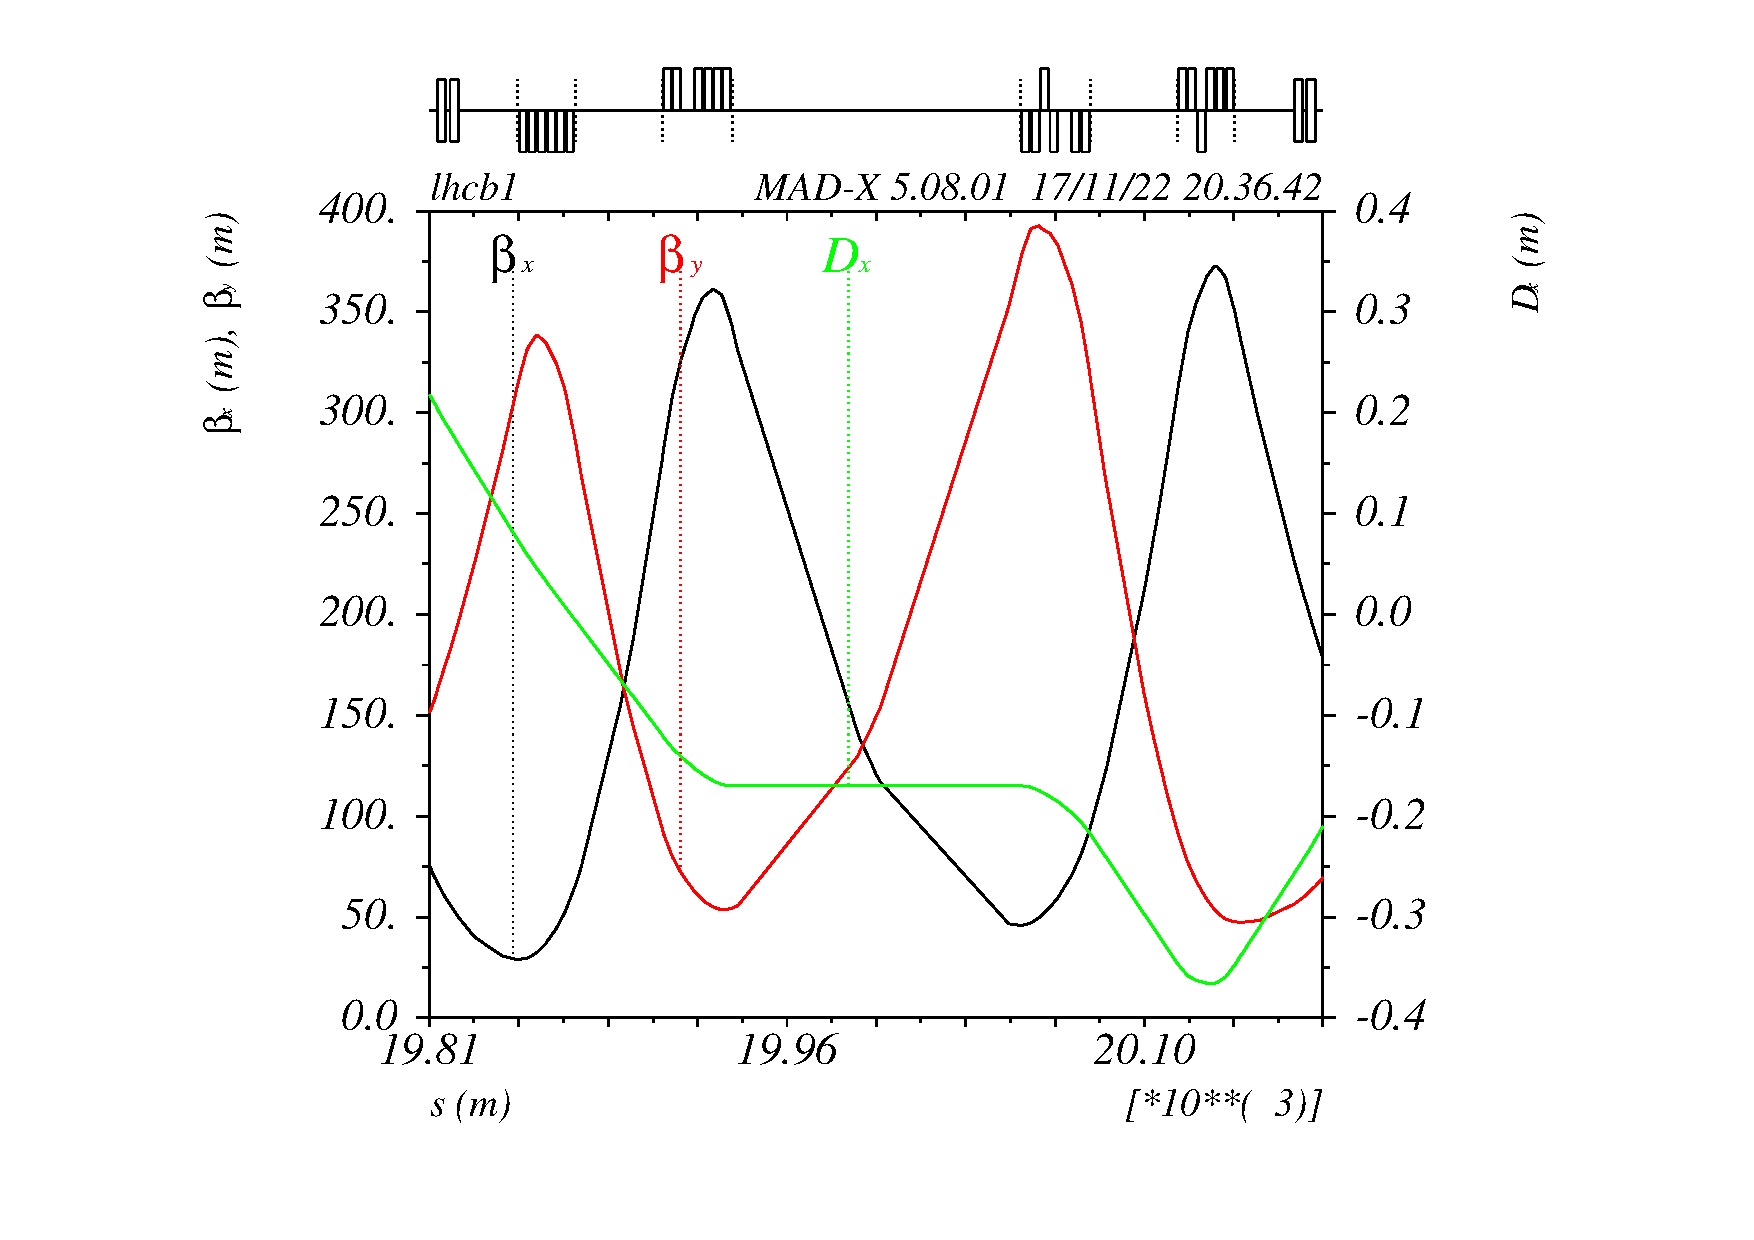
\includegraphics[width=0.76\linewidth, trim=85 45 70 15, clip]{plots/beam1/IR7_Run2.pdf}  
  \caption{Run 2}
\end{subfigure}
\begin{subfigure}{1.\textwidth}
  \centering
  % include second image
  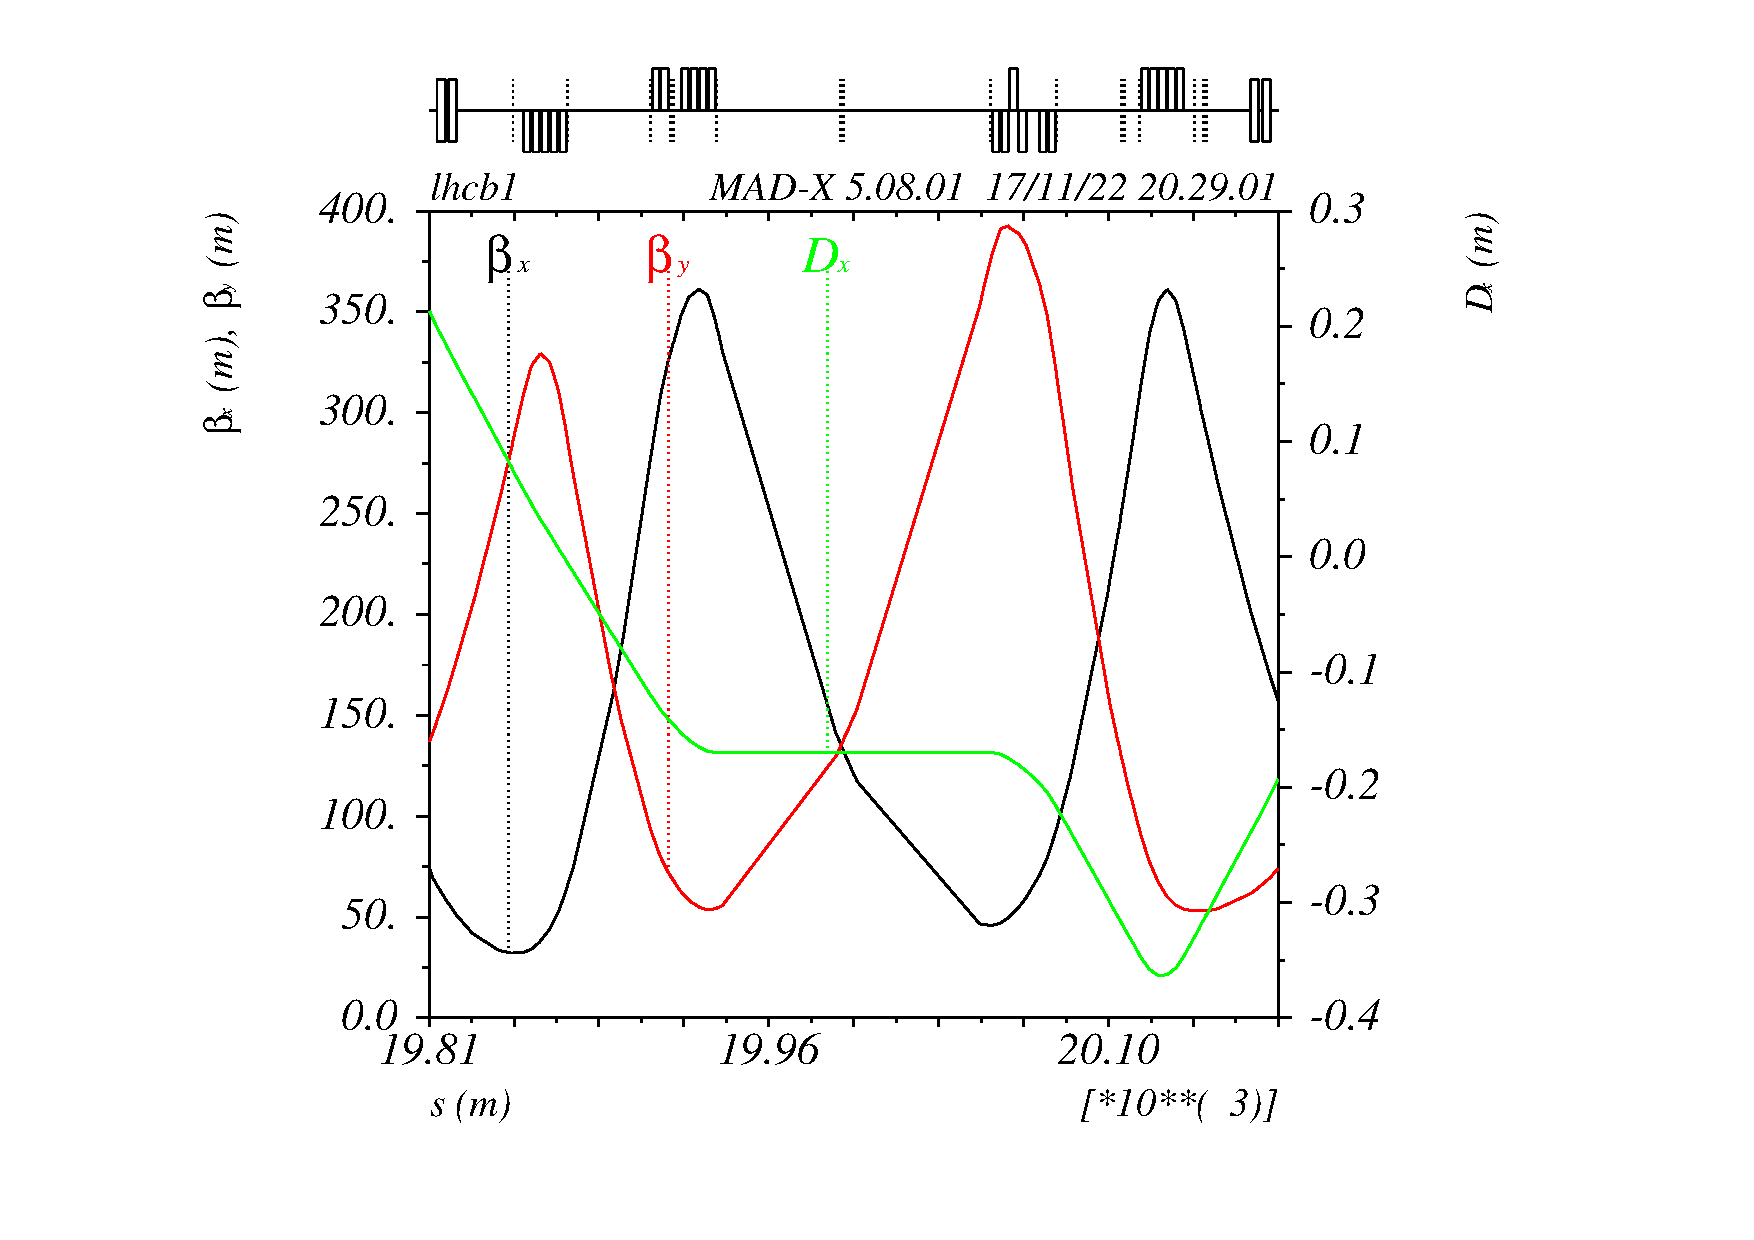
\includegraphics[width=.83\linewidth, trim=65 45 70 15, clip]{plots/beam1/IR7_Run3.pdf}  
  \caption{Run 3}
\end{subfigure}
\caption{IR7 layout and Beam 1 optics for Run~2 and Run~3. The rightmost and leftmost quadrupole blocks (Q5) have one fewer MQW (5 instead of 6) in Run 3 with a negligible impact on the optics functions.}
\label{fig:IR7}
\end{figure}


\section{Linear optics commissioning}
The beam test week took place in the autumn of 2021 with the intention of testing the LHC after the LS2 to be ready for the full restart in 2022.
The initial measurement of the $\beta$-beat showed significantly higher values than what was measured previously during commissioning. This is shown in Fig.~\ref{fig:initalVs2016} for Beam~1 and Beam~2 respectively.  


\begin{figure}[ht]
\begin{subfigure}{.5\textwidth}
  \centering
  % include first image
  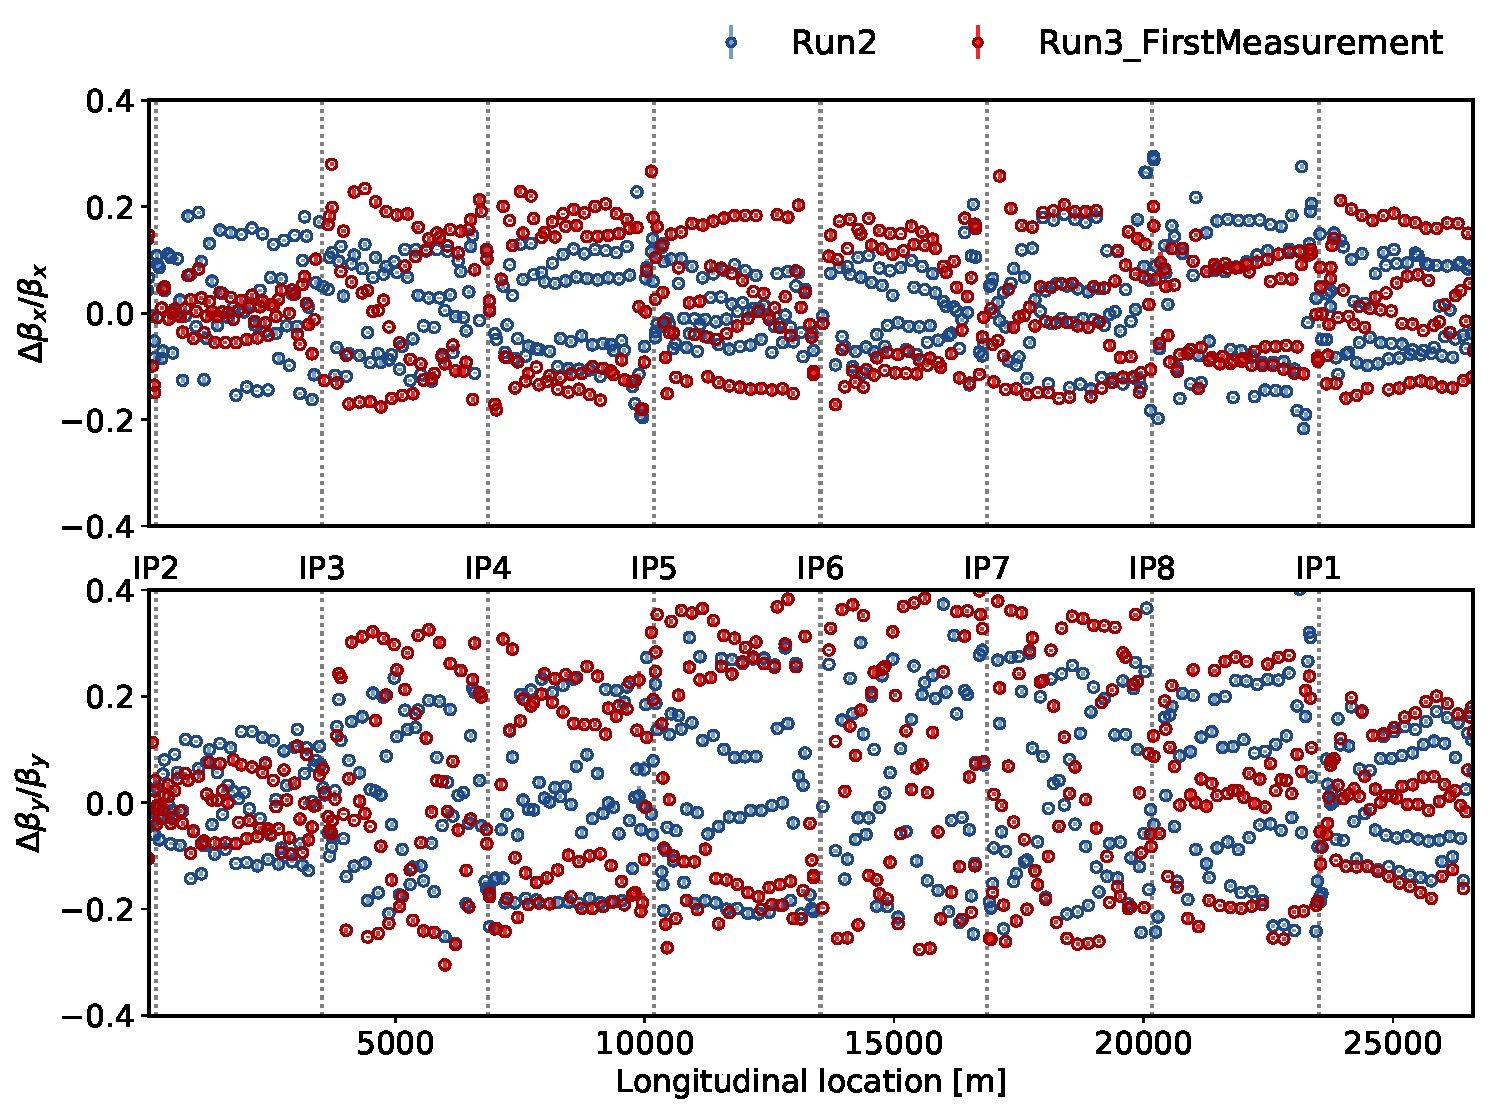
\includegraphics[width=.8\linewidth]{plots/beam1/beta_beat_virgin_2016_2021.pdf}  
  \caption{Beam~1}
\end{subfigure}
\begin{subfigure}{.5\textwidth}
  \centering
  % include second image
  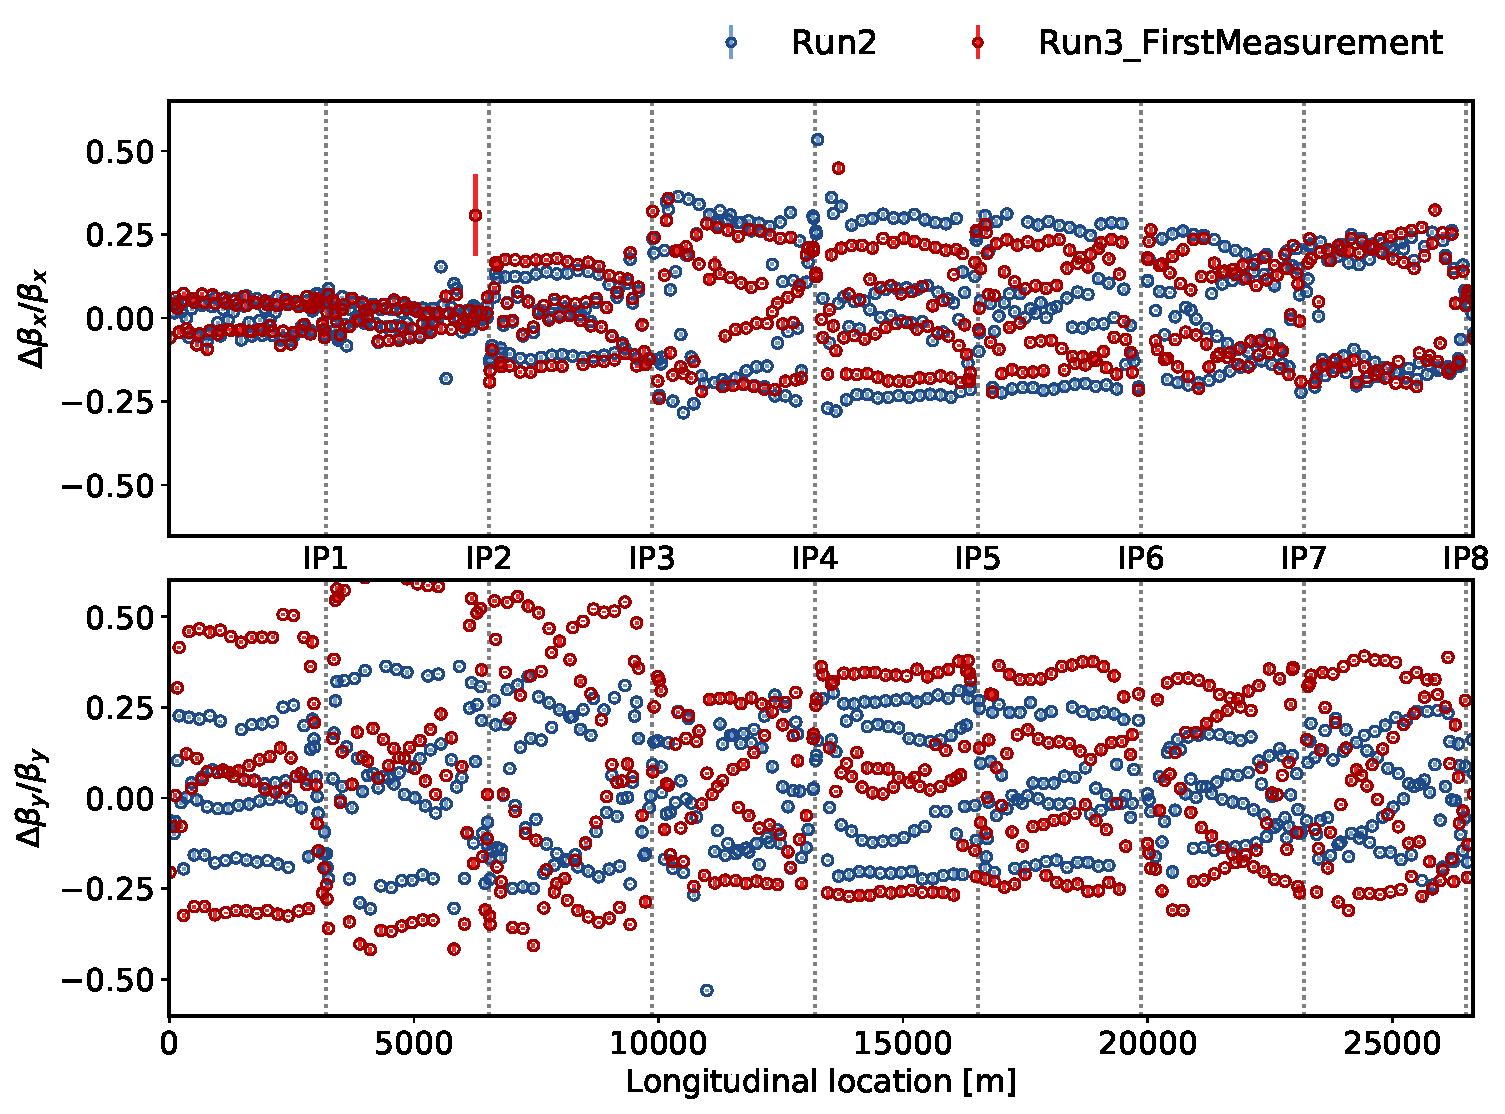
\includegraphics[width=.8\linewidth]{plots/beam2/B2_BetaBeat_2016_vs_first2021.pdf}  
  \caption{Beam~2}
\end{subfigure}
\caption{The $\beta$-beating for the first measurement in 2021 compared to the measurement in 2016 (during MD).}
\label{fig:initalVs2016}
\end{figure}
%beta_beat_before_after_pre_beam1.pdf

The first attempt was to try to understand if something had gone wrong during the pre-cycle or the fact that the machine had been around 40h at injection without any pre-cycle could have an effect. The re-measurement showed a modest effect on the $\beta$-beat as seen in Fig.~\ref{fig:before_after_pre_cycle}. This is a positive results since a big change of the $\beta$-beat at injection would have meant that long fills at injection should be avoided. 

\begin{figure}[ht]
\begin{subfigure}{.5\textwidth}
  \centering
  % include first image
  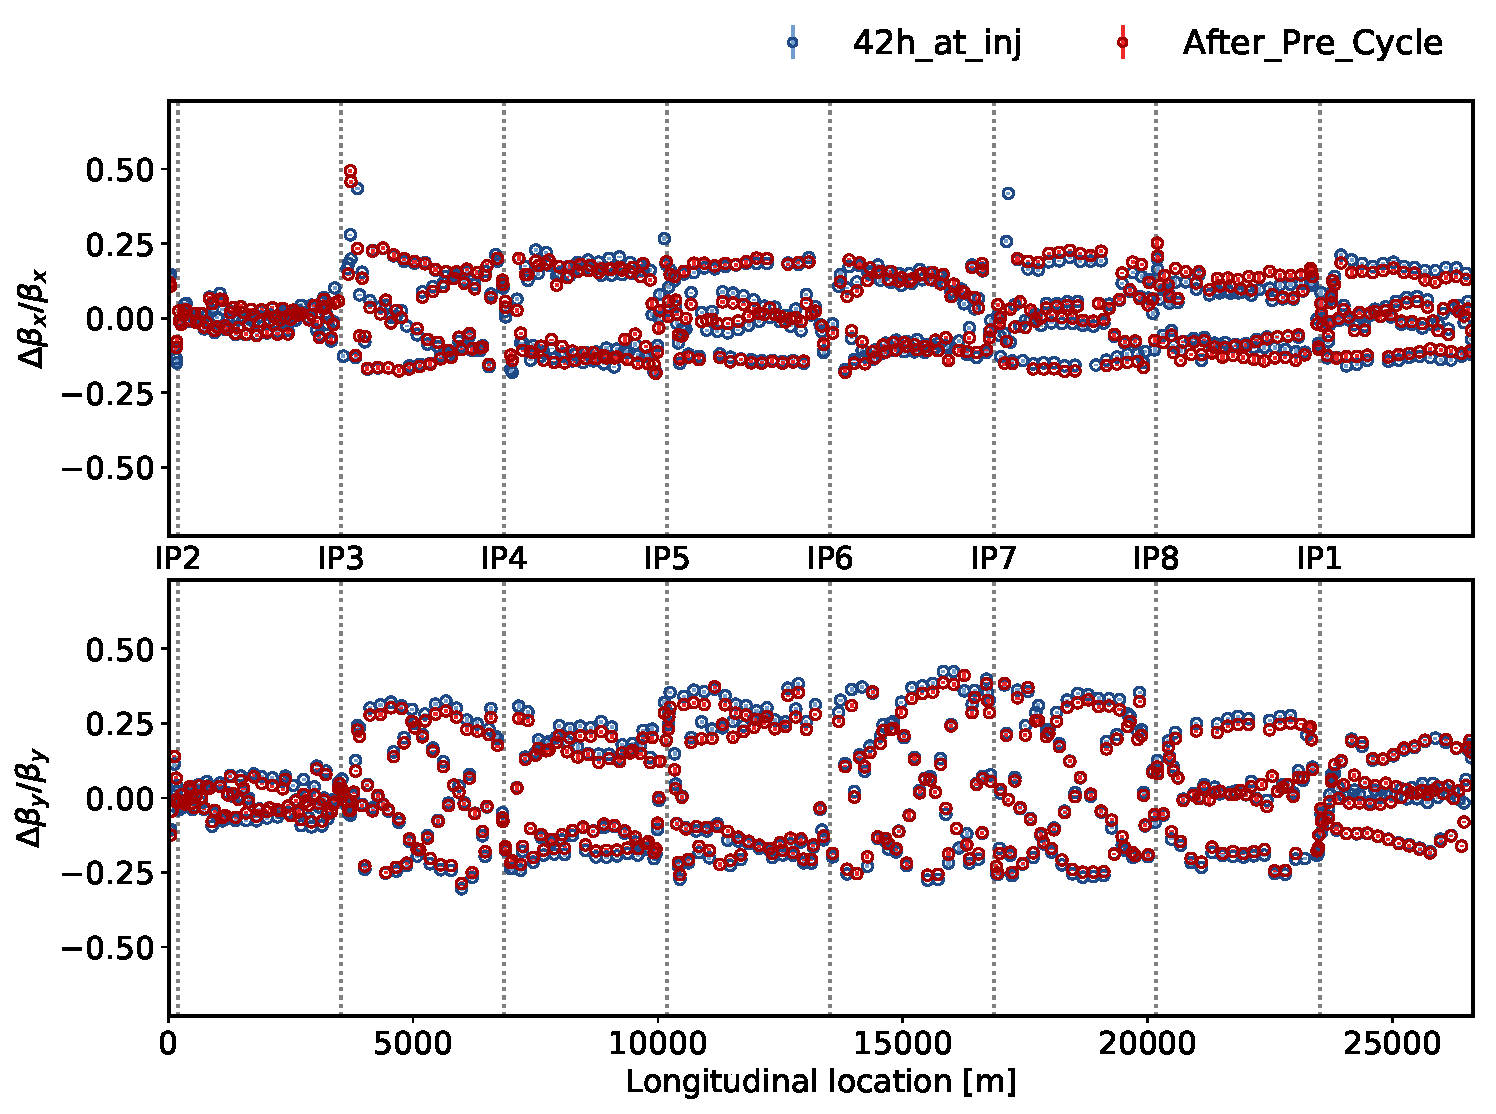
\includegraphics[width=.8\linewidth]{plots/beam1/beta_beat_before_after_pre_beam1.pdf}  
  \caption{Beam~1}
\end{subfigure}
\begin{subfigure}{.5\textwidth}
  \centering
  % include second image
  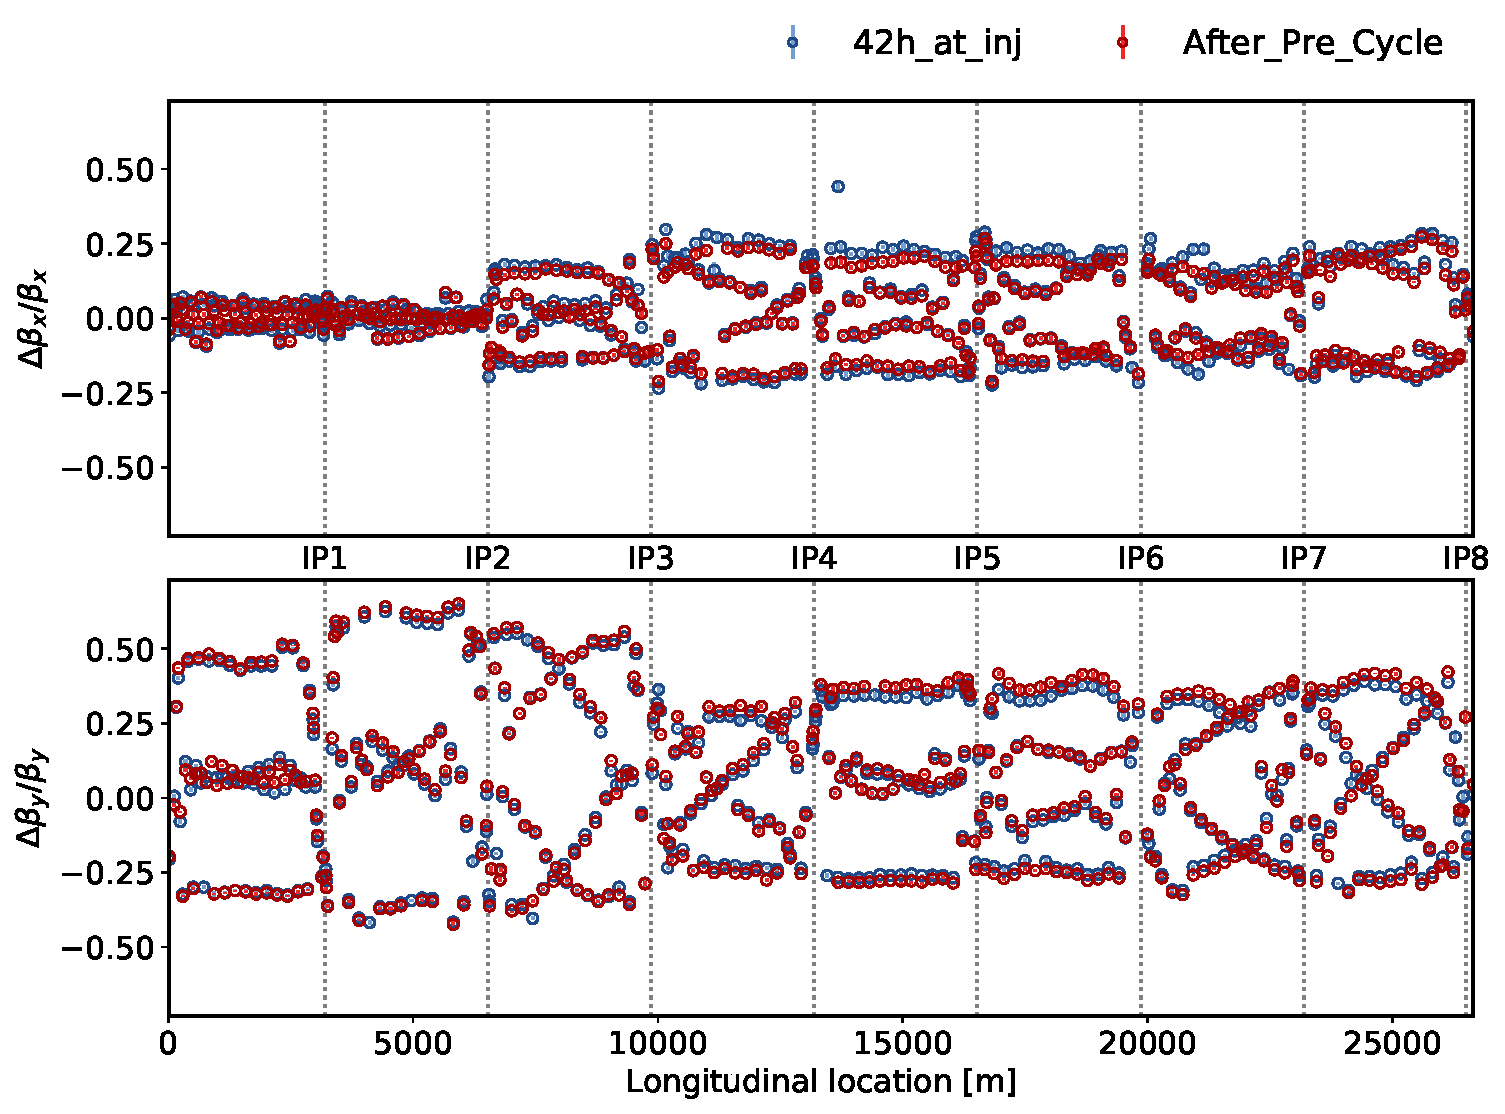
\includegraphics[width=.8\linewidth]{plots/beam2/beta_beat_before_after_pre_beam2.pdf}  
  \caption{Beam~2}
\end{subfigure}
\caption{A comparison of before and after the pre-cycle.}
\label{fig:before_after_pre_cycle}
\end{figure}


After ruling out that the big change was coming coming from the extended time spent at injection we attempted to find the location of the error. Using the Segment-by-Segment (SBS)~\cite{first} technique it was found that there was a large phase deviation around IP3 and in particular around RQTL7.R3. It was decided that we should try to trim on that magnet in order to reduce the $\beta$-beat. The first observation was that nothing changed at all (not even a tune change). We then observed that the tune was changing on the opposite beam. We then repeated the test for the RQTL7.R3 of the opposite beam and we then again observed a change in tune, again on the opposite beam. From that we could conclude that indeed the RQTL7.R3 were swapped. This was then traced to an old swap already detected in Run~1. This was fixed at that time but then during the LS2 it was again re-introduced~\ref{first, michiEvian}. After this was corrected on the software side a new measurement was carried out and the $\beta$-beat is shown in Fig.~\ref{fig:before_after_swap}. In this plot we can see that the $\beta$-beat was significantly reduced, as expected, after the swap was corrected.  

\begin{figure}[ht]
\begin{subfigure}{.5\textwidth}
  \centering
  % include first image
  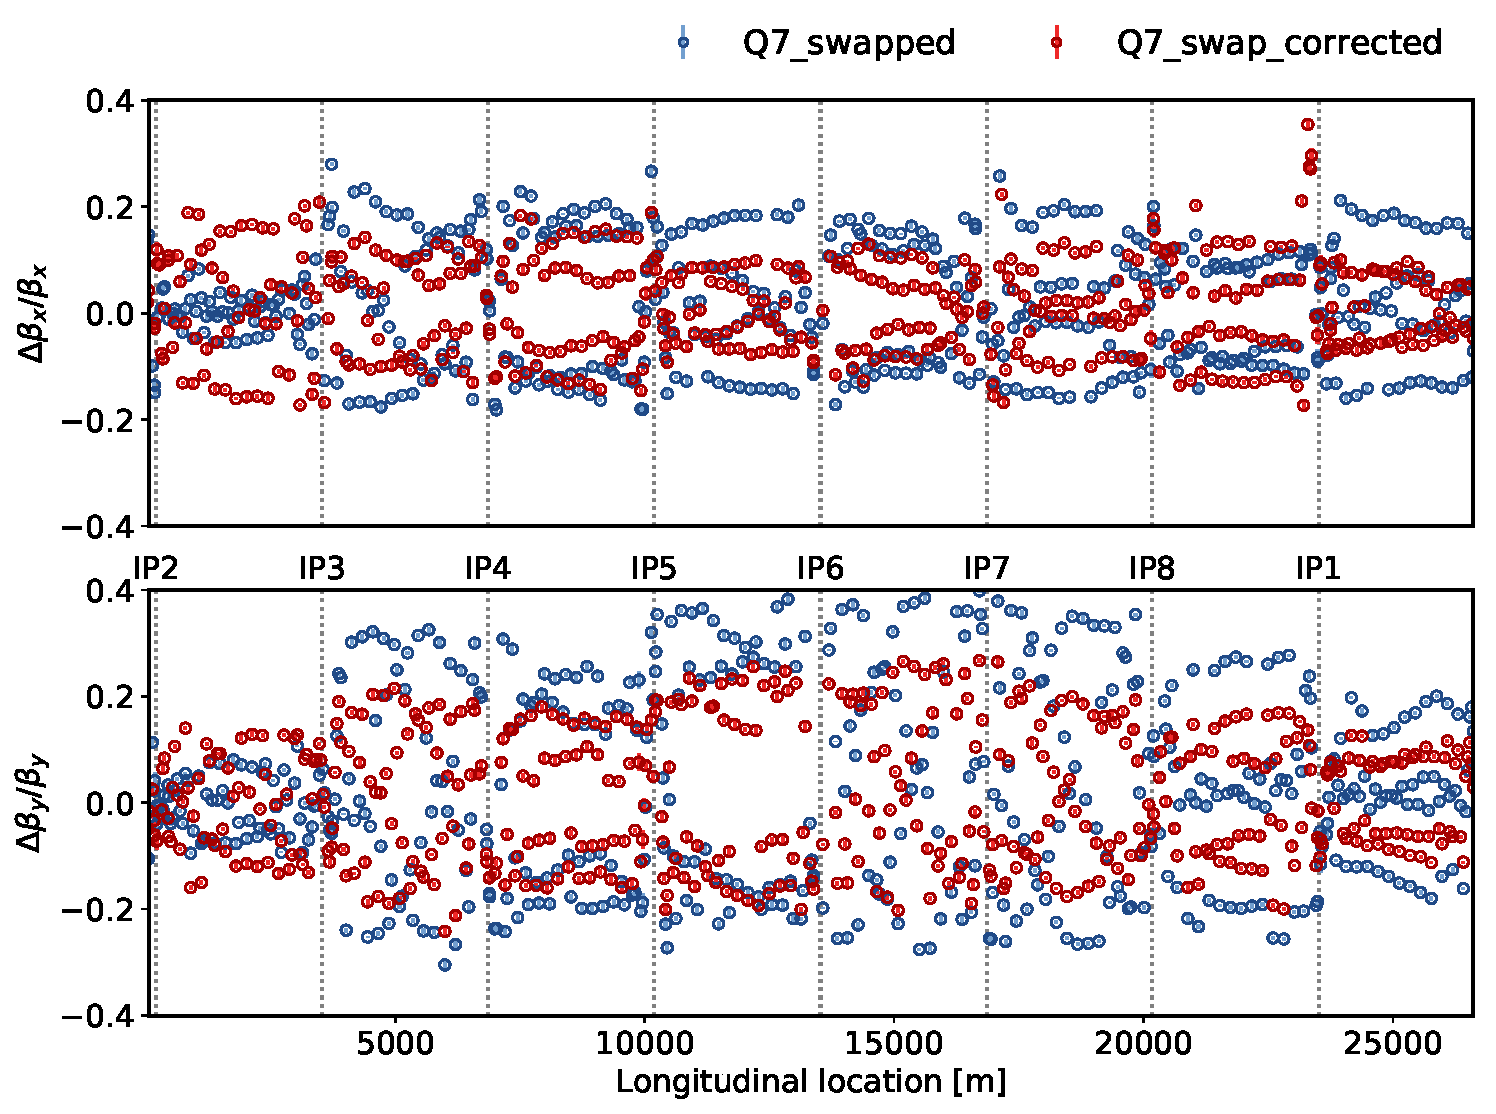
\includegraphics[width=.8\linewidth]{plots/beam1/beta_beat_before_after_swap.pdf}  
  \caption{Beam~1}
\end{subfigure}
\begin{subfigure}{.5\textwidth}
  \centering
  % include second image
  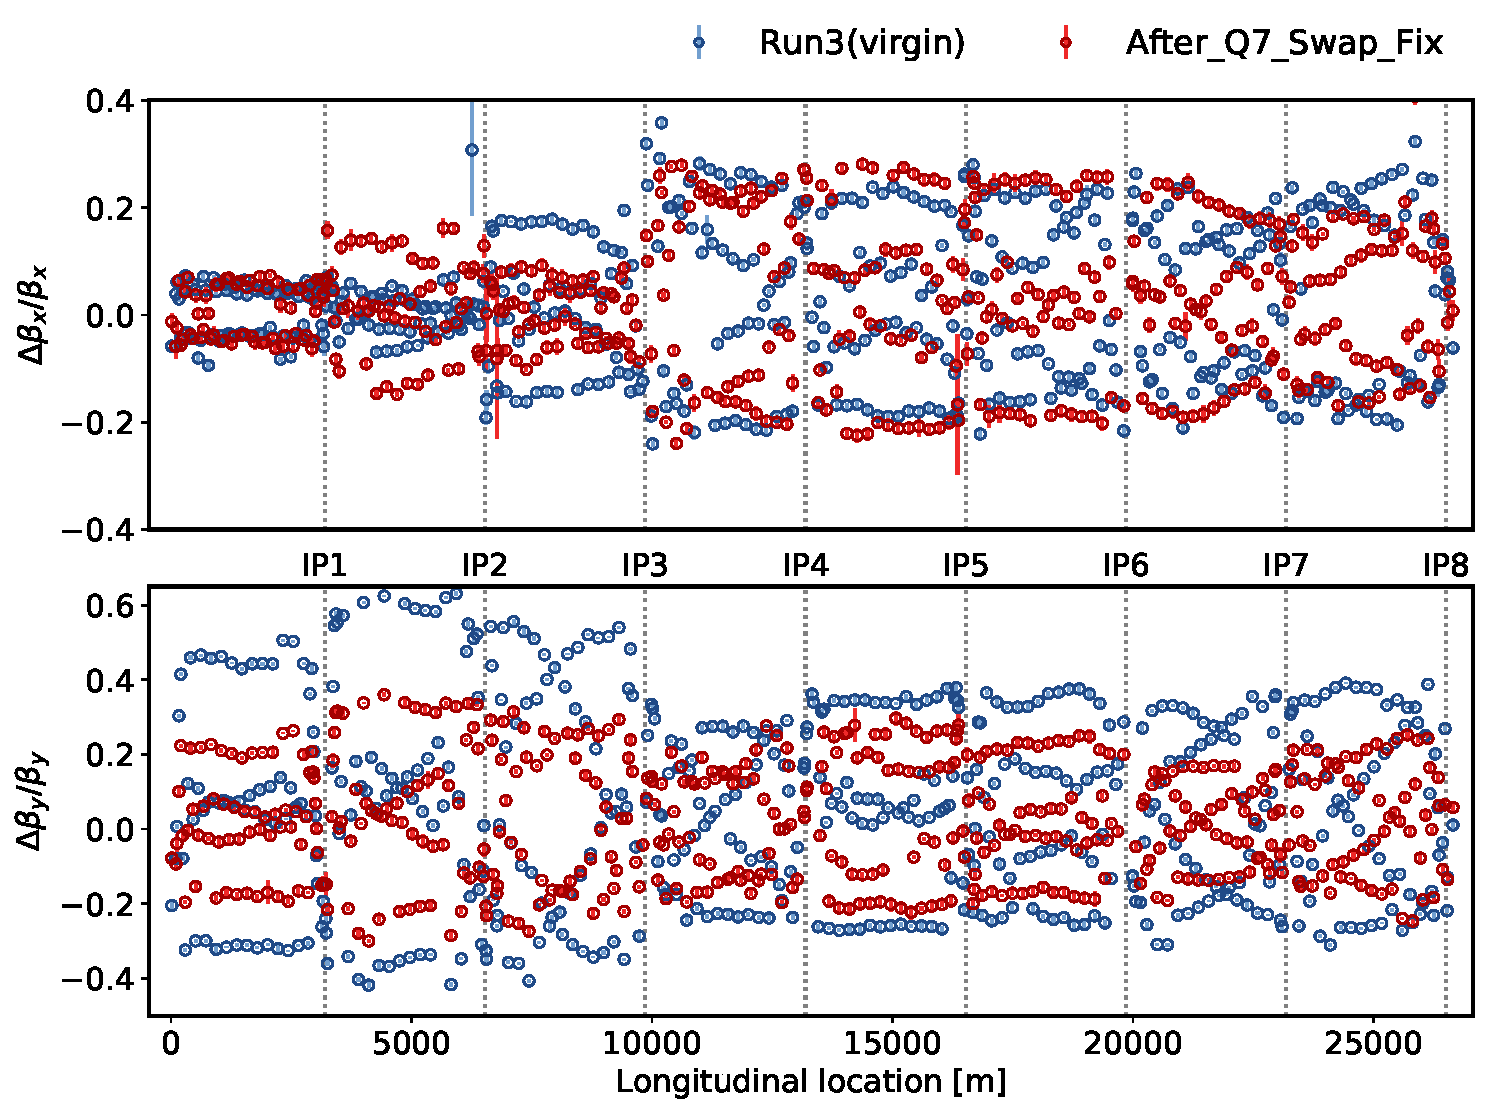
\includegraphics[width=.8\linewidth]{plots/beam2/beta_beat_before_vs_after_Q7_swap.pdf}  
  \caption{Beam~2}
\end{subfigure}
\caption{A comparison of before and after correcting the swap of the RQTL7.R3.}
\label{fig:before_after_swap}
\end{figure}

It is also interesting to observe if there is any sign of any degradation or any other major changes in the machine compared to Run~2. A such comparison is shown in Fig.~\ref{fig:after_swap_vs_2016}. We observe that the $\beta$-beat is similar between the two measurements and the small differences can be explained from the slightly different optics and change of a few of the dipoles. 

\begin{figure}[ht]
\begin{subfigure}{.5\textwidth}
  \centering
  % include first image
  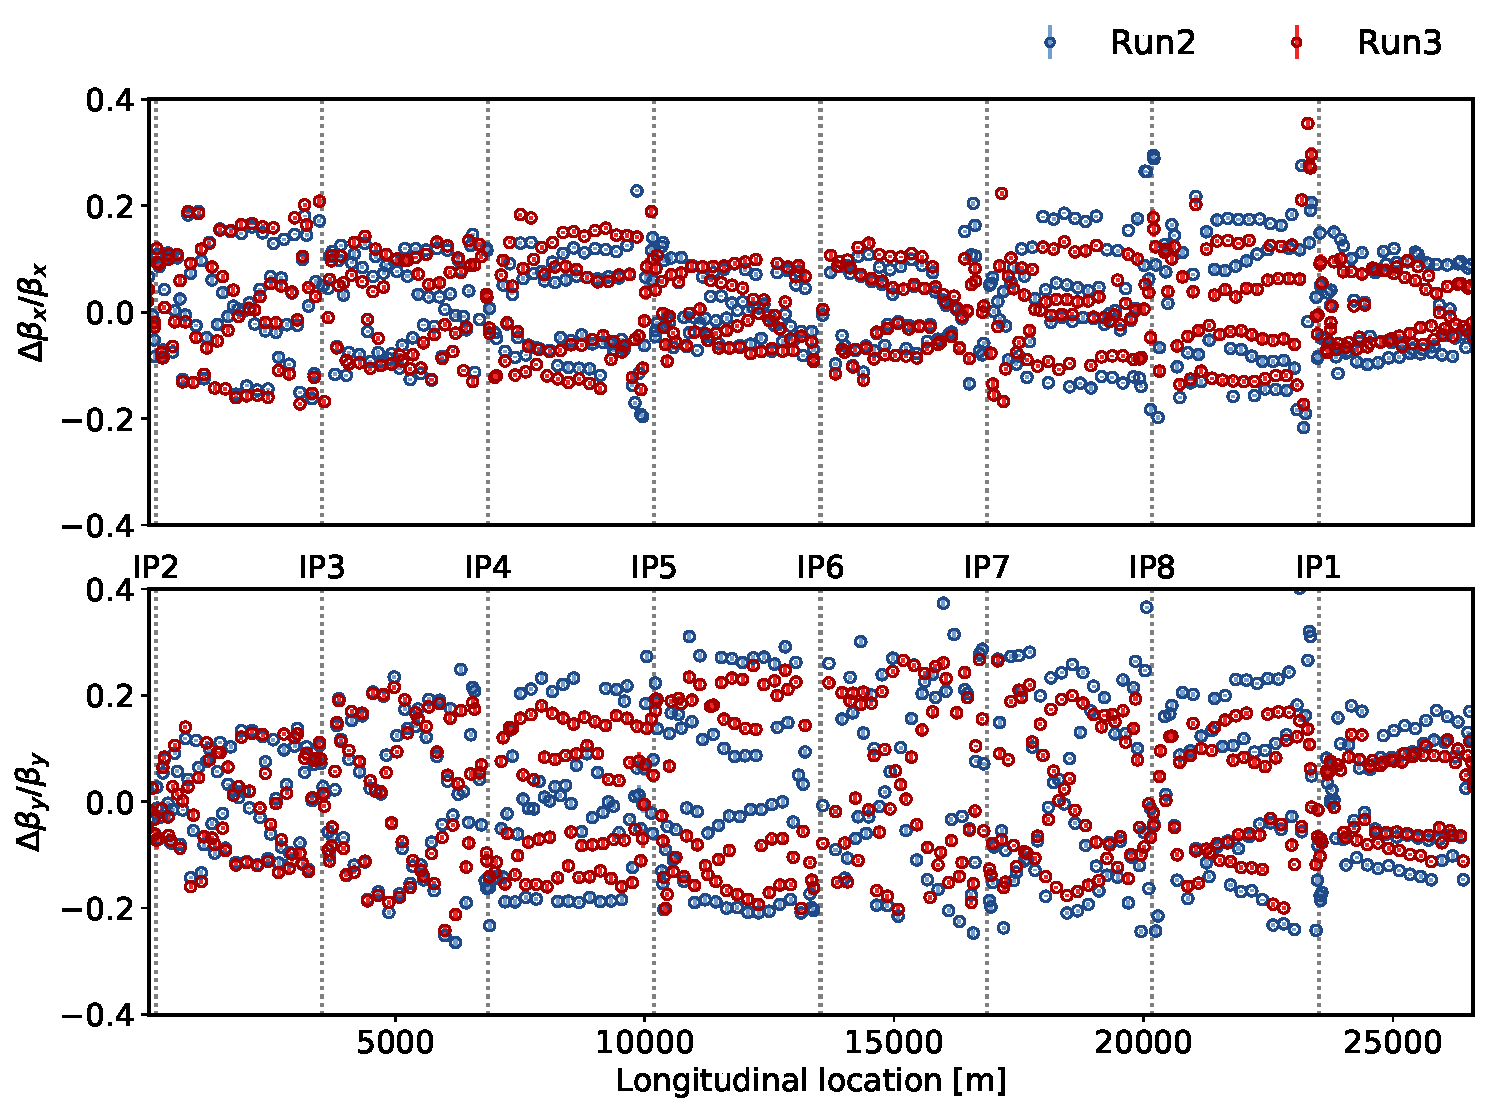
\includegraphics[width=.8\linewidth]{plots/beam1/beta_beat_2016_2021_swap_fixed.pdf}   
  \caption{Beam~1}
\end{subfigure}
\begin{subfigure}{.5\textwidth}
  \centering
  % include second image
  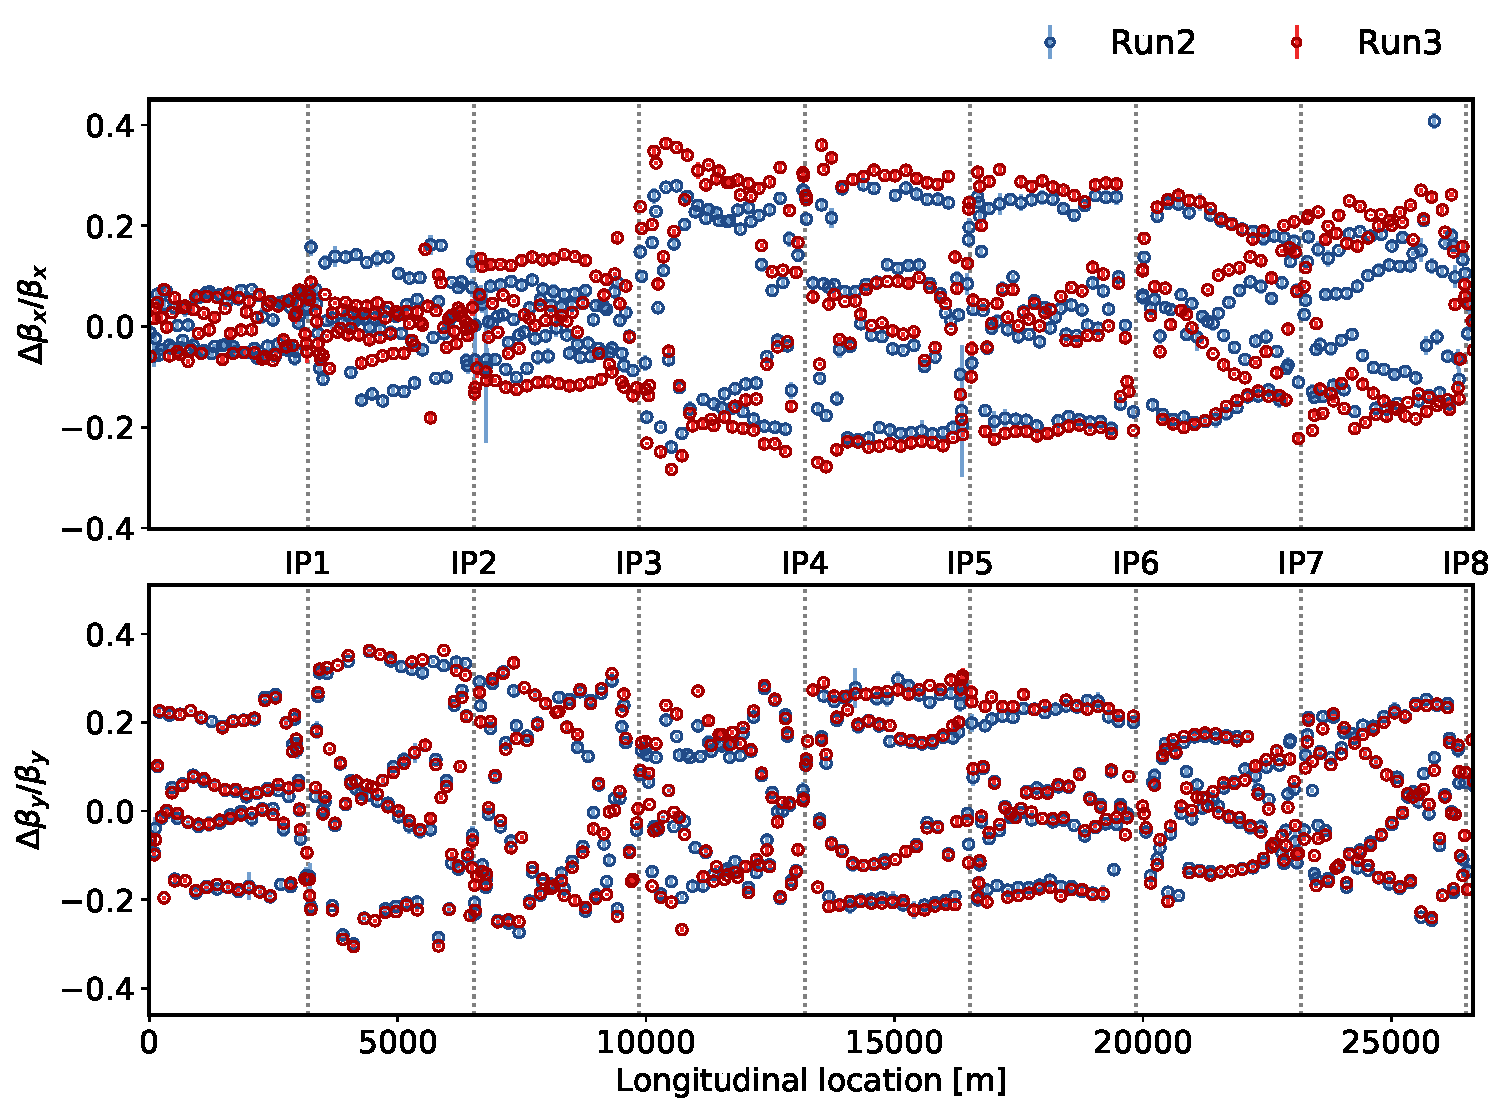
\includegraphics[width=.8\linewidth]{plots/beam2/B2_BetaBeat_afterIR3Q7fix_vs_virgin2016.pdf}
  \caption{Beam~2}
\end{subfigure}
\caption{After fix of swap of RQTL7.R3 vs Run~2 virgin injection optics.}
\label{fig:after_swap_vs_2016}
\end{figure}

Based on the measurement after the correction of the swapped quadrupole a correction of the phase advance as well as the normalized dispersion was calculated. The impact on the $\beta$-beat is shown in Fig.~\ref{fig:before_after_correction_beta_beat} and the impact on the normalized dispersion is shown in Fig.~\ref{fig:before_after_correction_beta_beat}. 

\begin{figure}[ht]
\begin{subfigure}{.5\textwidth}
  \centering
  % include first image
  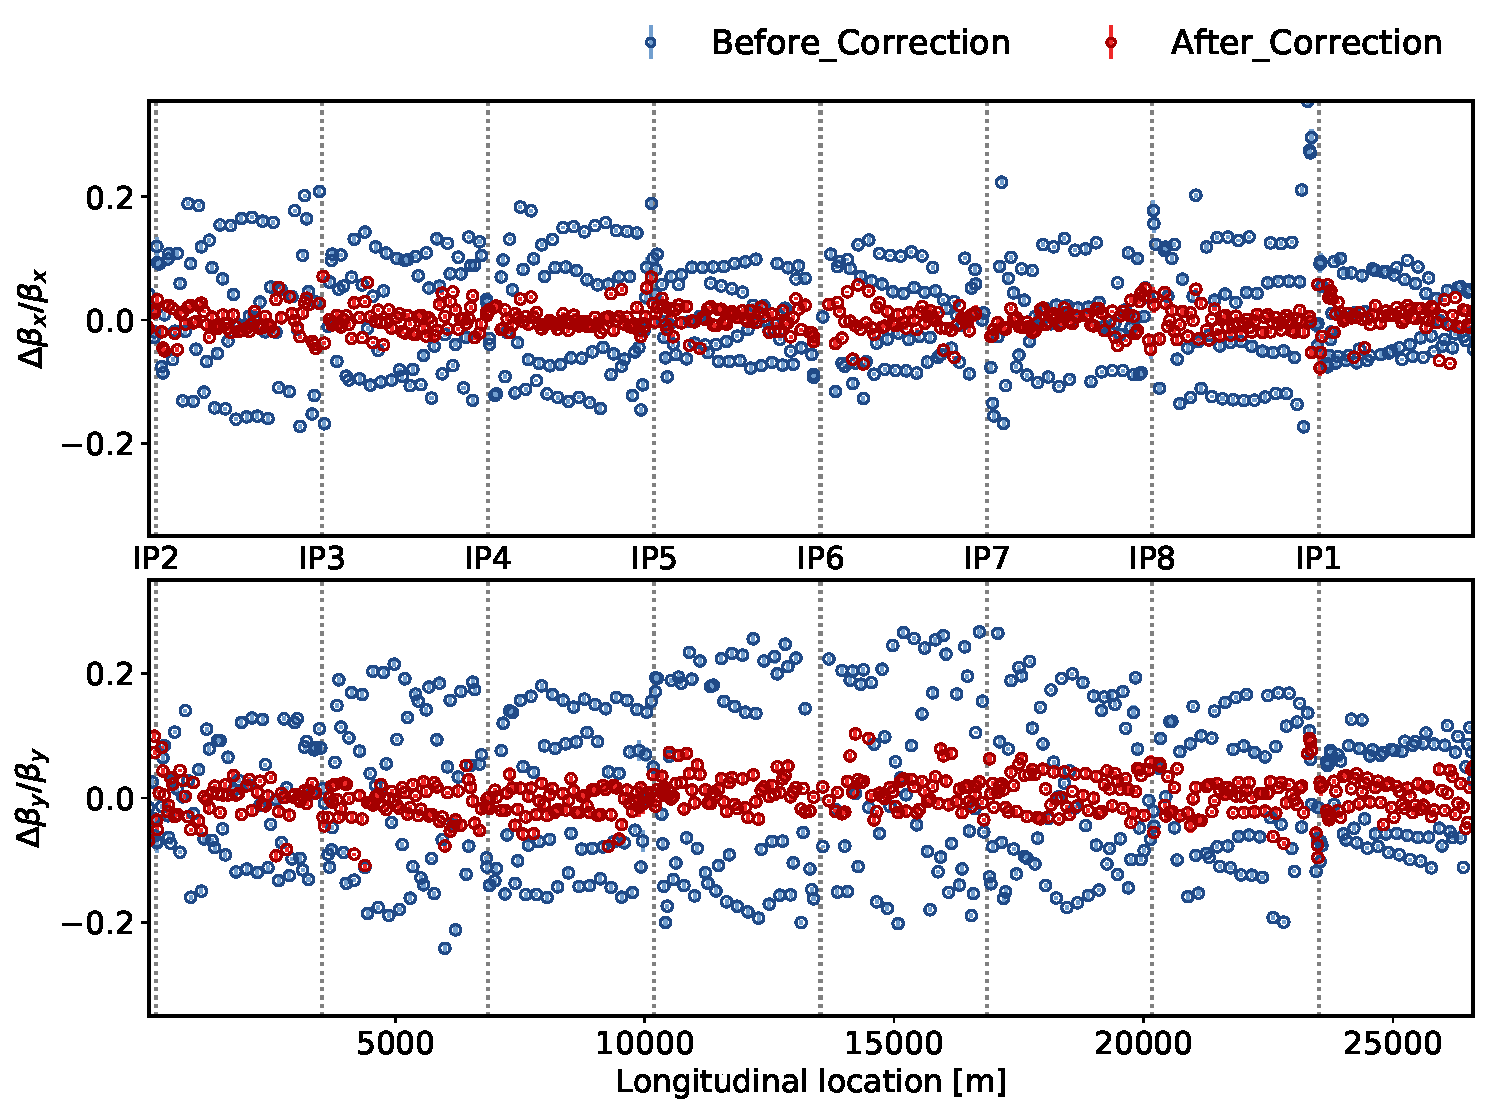
\includegraphics[width=.8\linewidth]{plots/beam1/beta_beat_before_and_after_corr.pdf}  
  \caption{Beam~1}
\end{subfigure}
\begin{subfigure}{.5\textwidth}
  \centering
  % include second image
  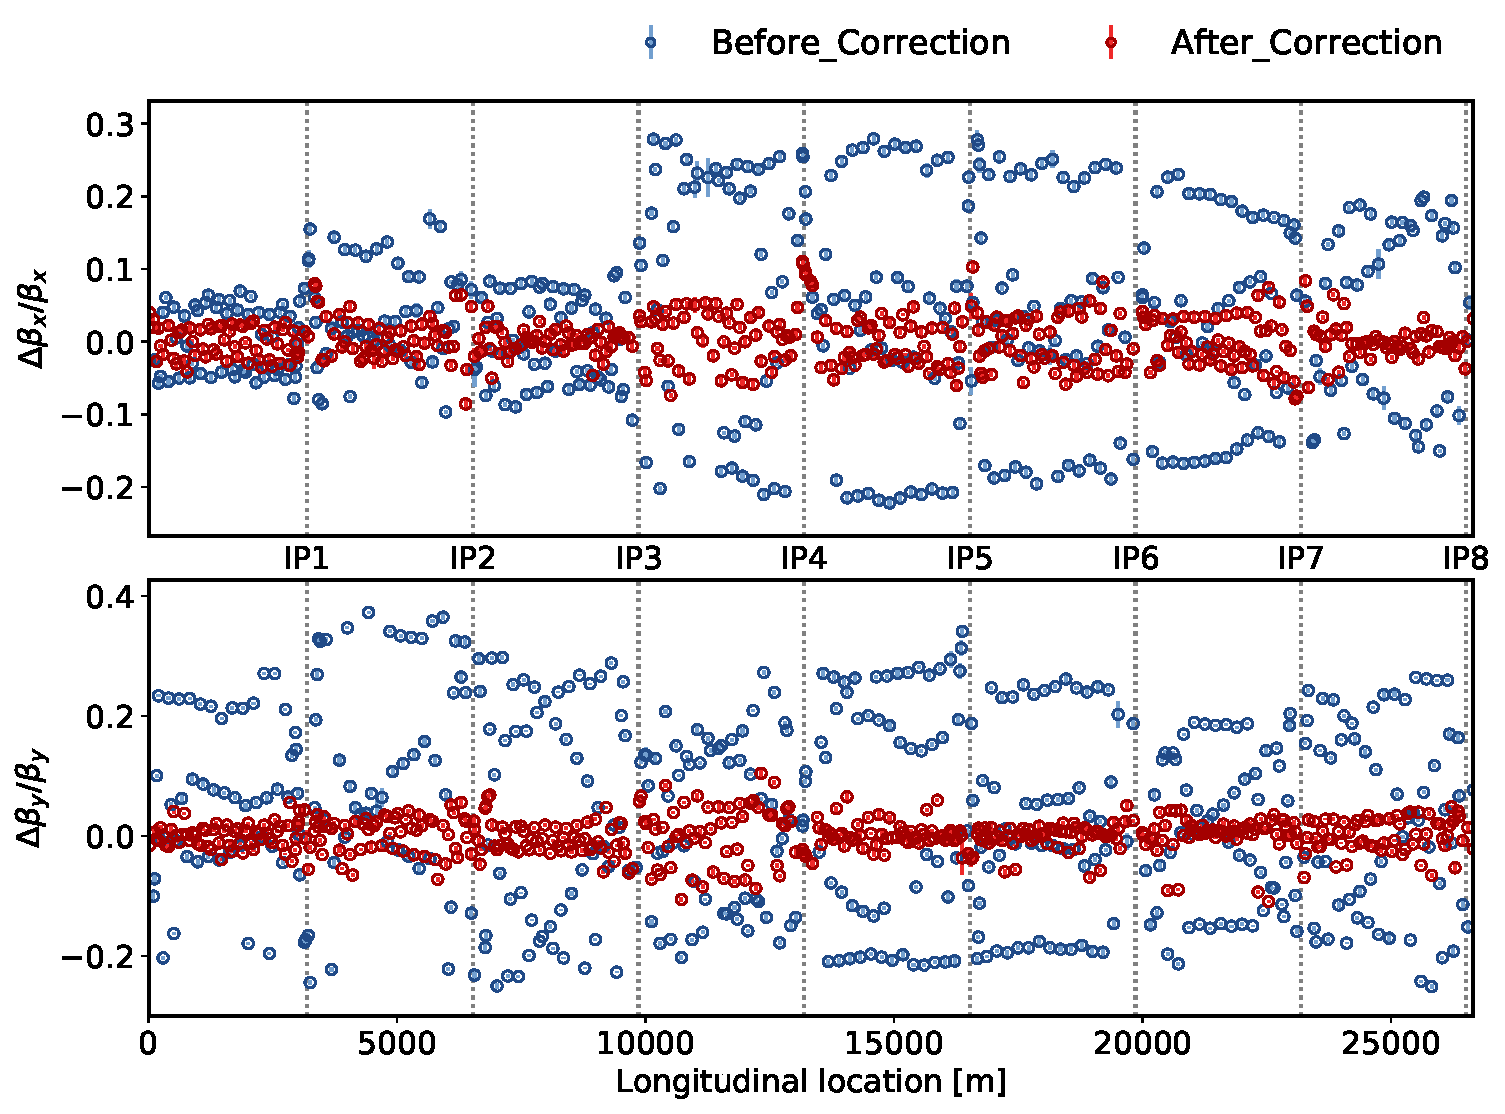
\includegraphics[width=.8\linewidth]{plots/beam2/beta_beat_before_after_correction.pdf}  
  \caption{Beam~2}
\end{subfigure}
\caption{Beta-beat before and after correction.}
\label{fig:before_after_correction_beta_beat}
\end{figure}

\begin{figure}[ht]
\begin{subfigure}{.5\textwidth}
  \centering
  % include first image
  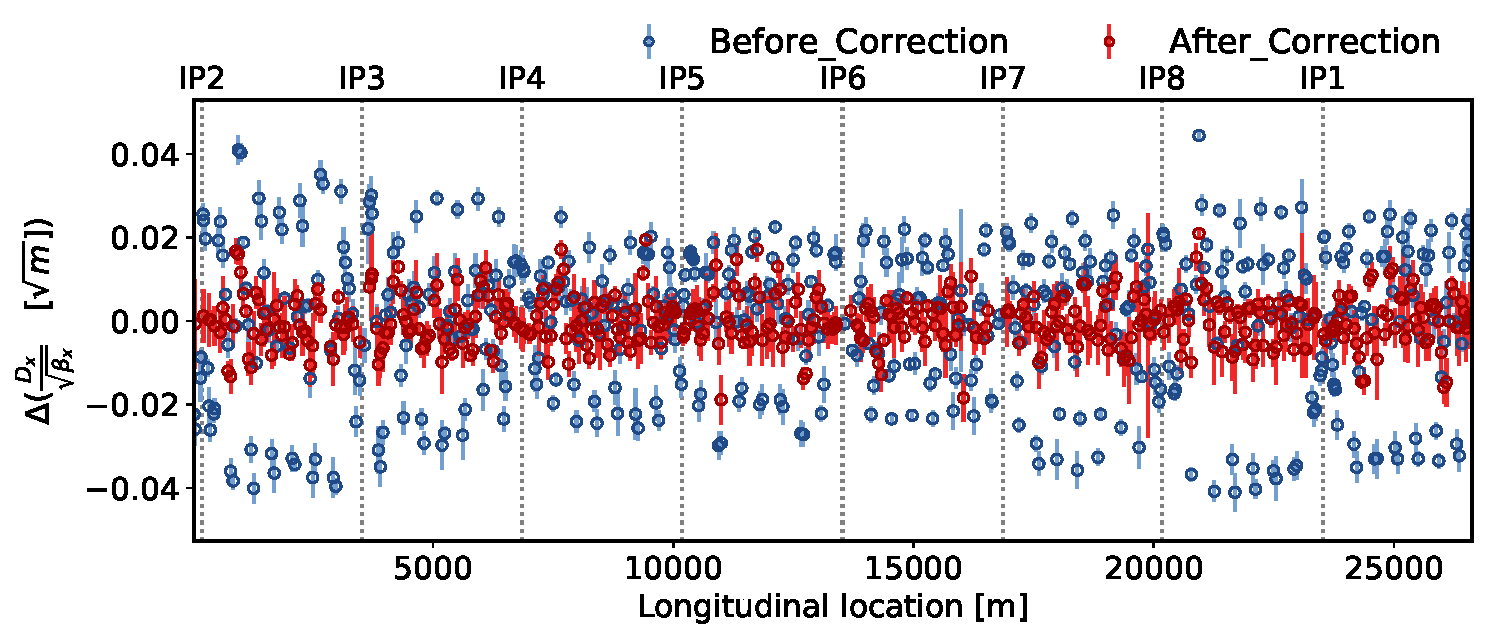
\includegraphics[width=.8\linewidth]{plots/beam1/Normalized_disp_before_vs_after_corection.pdf}  
  \caption{Beam~1}
\end{subfigure}
\begin{subfigure}{.5\textwidth}
  \centering
  % include second image
  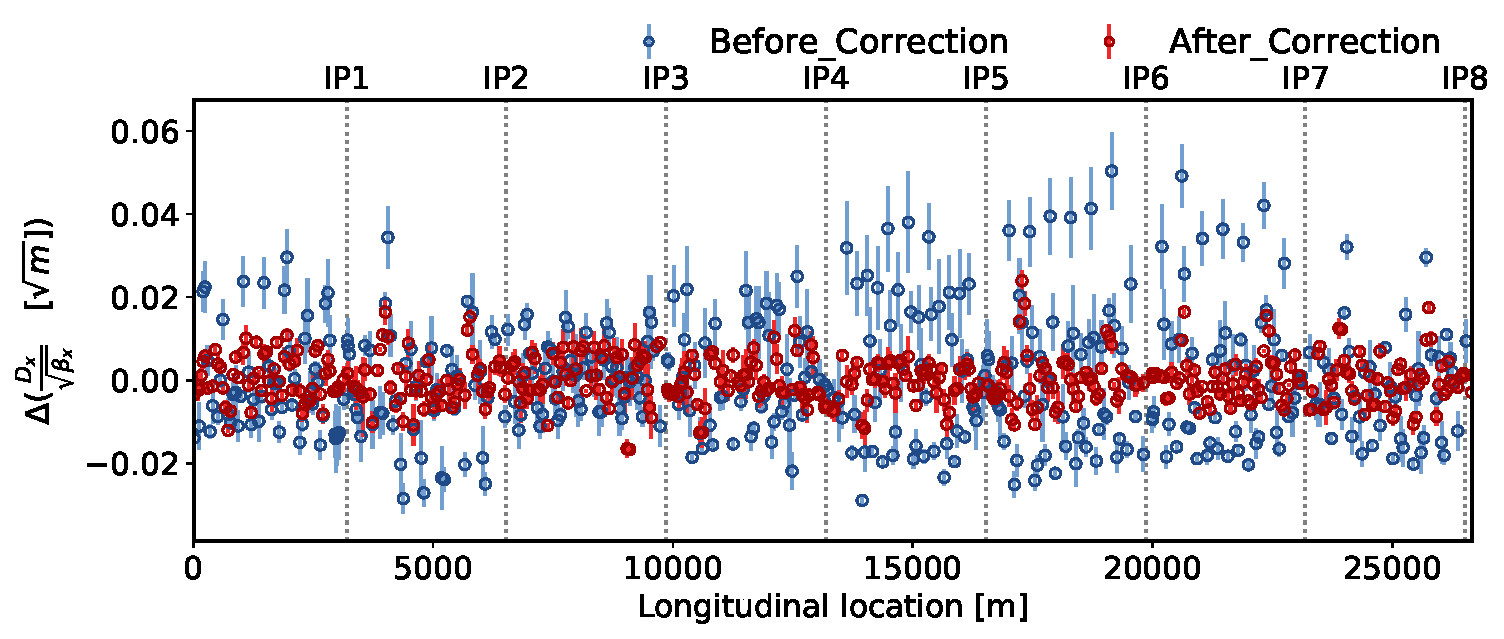
\includegraphics[width=.8\linewidth]{plots/beam2/ndisp_before_after_correction.pdf}  
  \caption{Beam~2}
\end{subfigure}
\caption{Normalized dispersion before and after correction.}
\label{fig:before_after_correction_beta_beat}
\end{figure}


In Fig~\ref{fig:2017_beta_beat_vs_2021} a comparision of the $beta$-beat in Run~2 compared to Run~3 is shown. We can see that the level of corrections is similar for the two runs with a slight improvement for Beam~1 in Run~3. 

\begin{figure}[ht]
\begin{subfigure}{.5\textwidth}
  \centering
  % include first image
  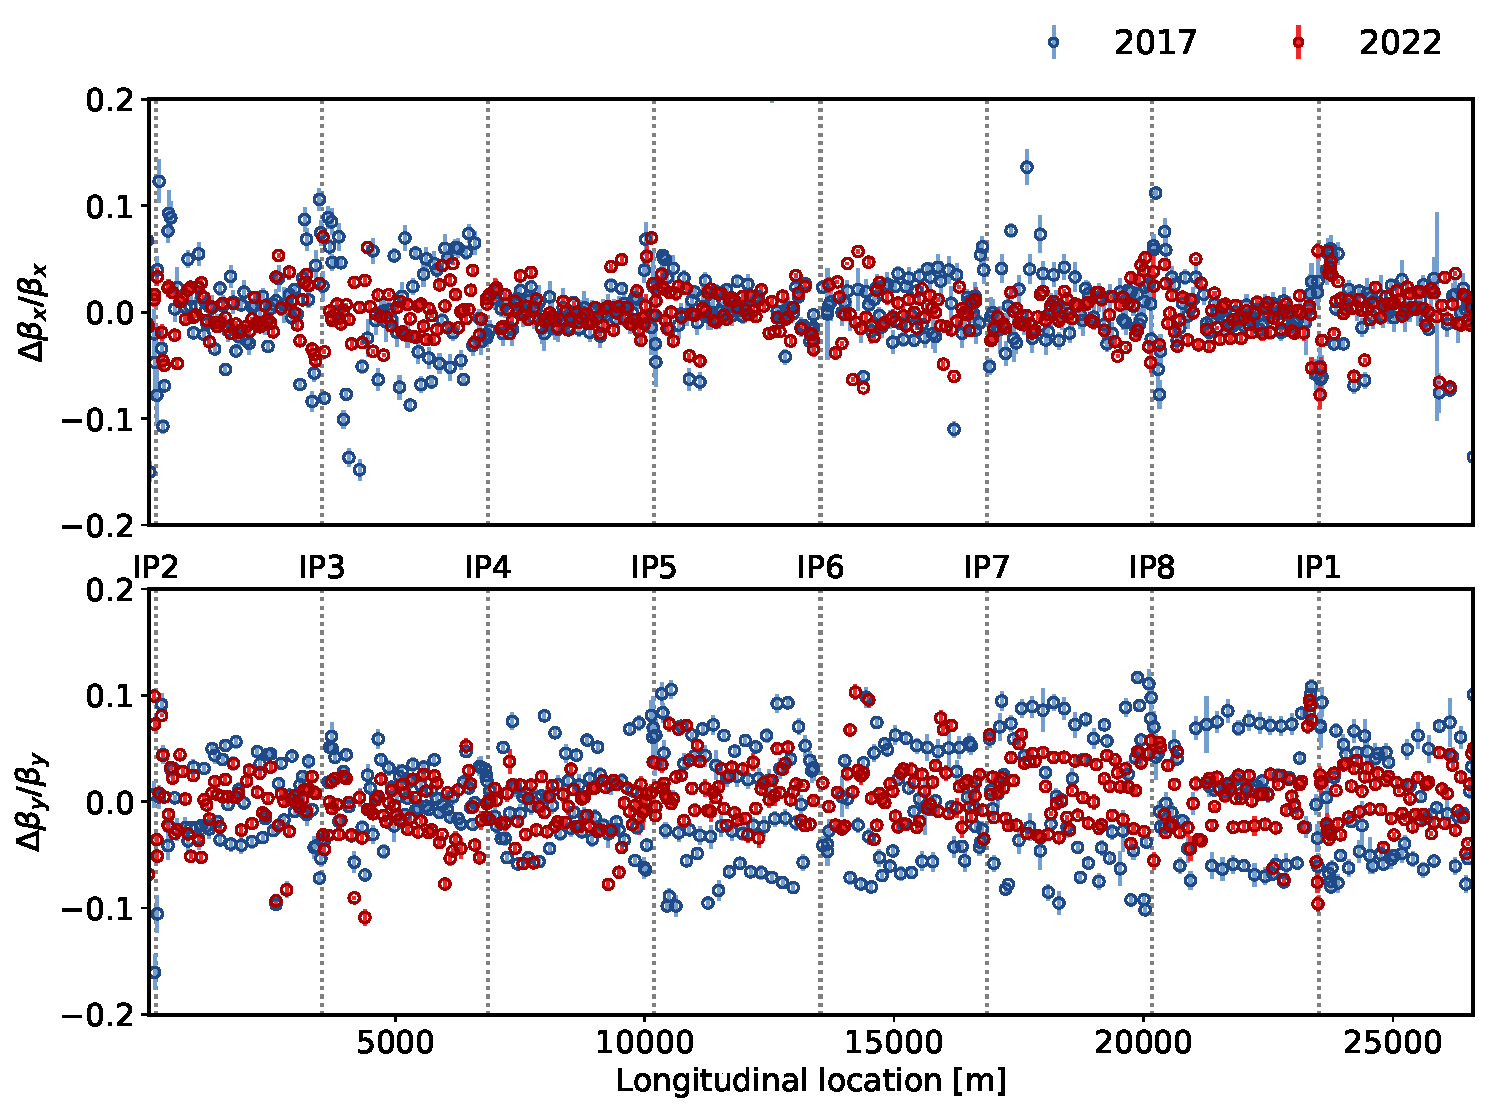
\includegraphics[width=.8\linewidth]{plots/beam1/after_corr_2017_vs_2021.pdf}  
  \caption{Beam~1}
\end{subfigure}
\begin{subfigure}{.5\textwidth}
  \centering
  % include second image
  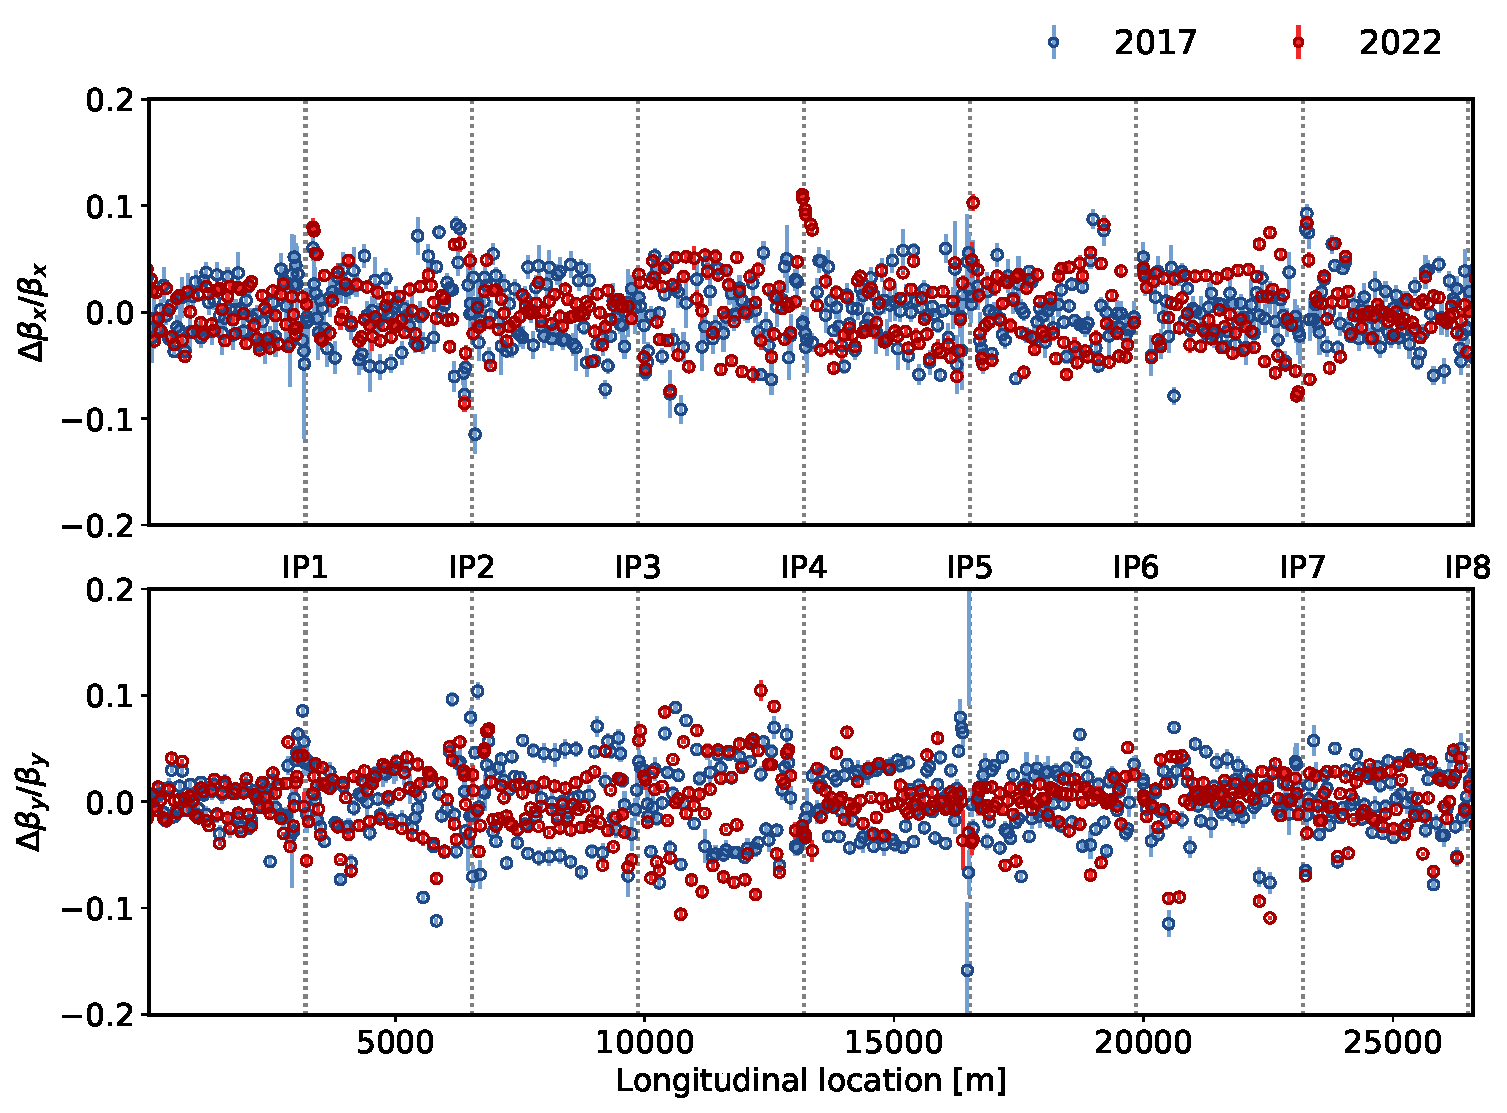
\includegraphics[width=.8\linewidth]{plots/beam2/after_corr_2017_vs_2021_beam2.pdf}  
  \caption{Beam~2}
\end{subfigure}
\caption{The $\beta$-beating measured after correction during the beam-test compared to what was measured at injection in 20107.}
\label{fig:2017_beta_beat_vs_2021}
\end{figure}

In Fig.~\ref{fig:corrector_strength_injection} the change in powering of the magnets to archive the corrections is shown. The maximum strength between the corrections used in Run~2 and Run~3 is very similar but fewer magnets were used for the Run~3 correction, in particular for Beam~1. This is due to slightly different settings were used to calculate the corrections.  

\begin{figure}[ht]
\begin{subfigure}{.5\textwidth}
  \centering
  % include first image
  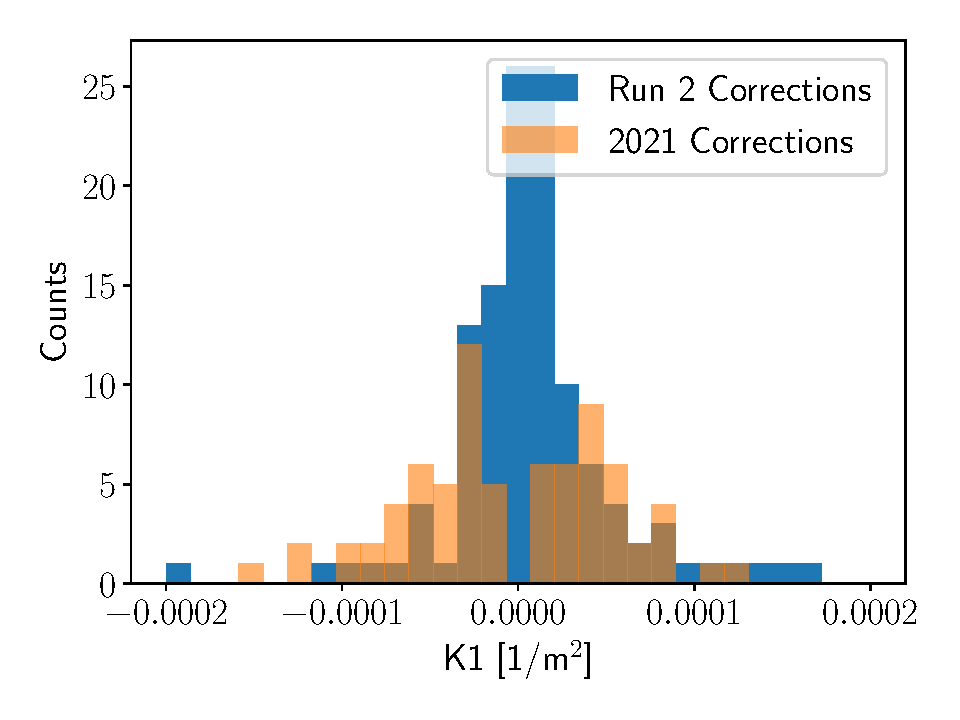
\includegraphics[width=.8\linewidth]{beam1_corrections.pdf}  
  \caption{Beam~1}
\end{subfigure}
\begin{subfigure}{.5\textwidth}
  \centering
  % include second image
  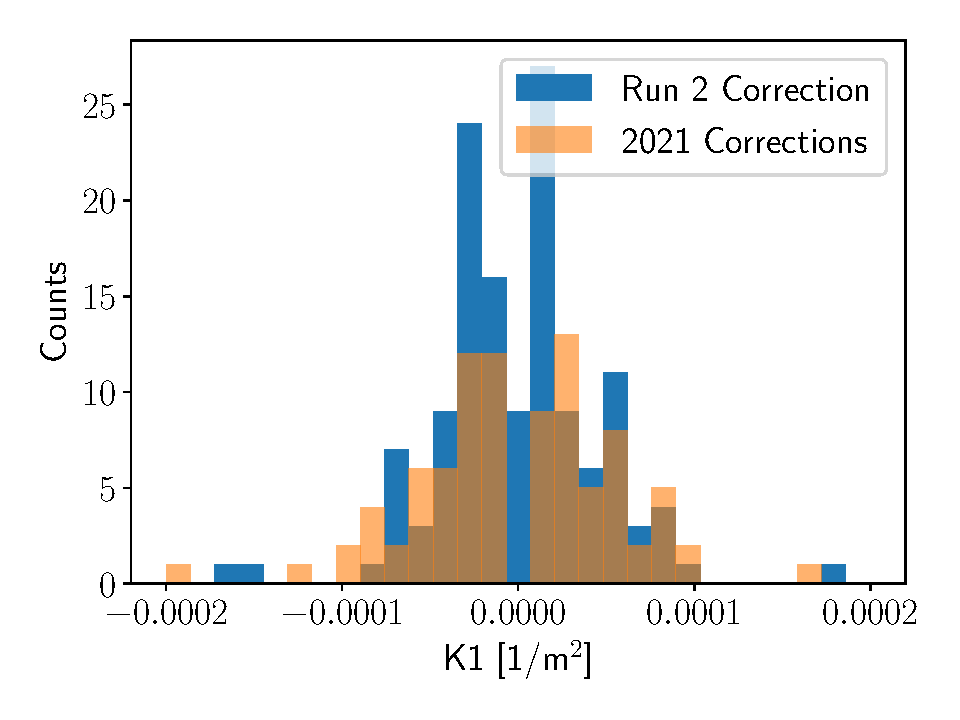
\includegraphics[width=.8\linewidth]{beam2_corrections.pdf}  
  \caption{Beam~2}
\end{subfigure}
\caption{The correction strength in Run~2 compared to Run~3.}
\label{fig:corrector_strength_injection}
\end{figure}





\subsection{Reproducible}
No dedicated corrections were applied for the injections optics after the beam-test. However, the optics was validated when the machine was again switched on in 2022. In Fig.~\ref{fig:} a comparison of the $\beta$-beat measured during the beam test compared to what was measured in April 2021 in the beginning of the optics commissioning. We can observe that while Beam~1 seems to have a very similar pattern and max value Beam~2 shows a slight increase. The increase was, however, small enough to not be considered to be an issue and was therefore left without any additional corrections. 


\begin{figure}[ht]
\begin{subfigure}{.5\textwidth}
  \centering
  % include first image
  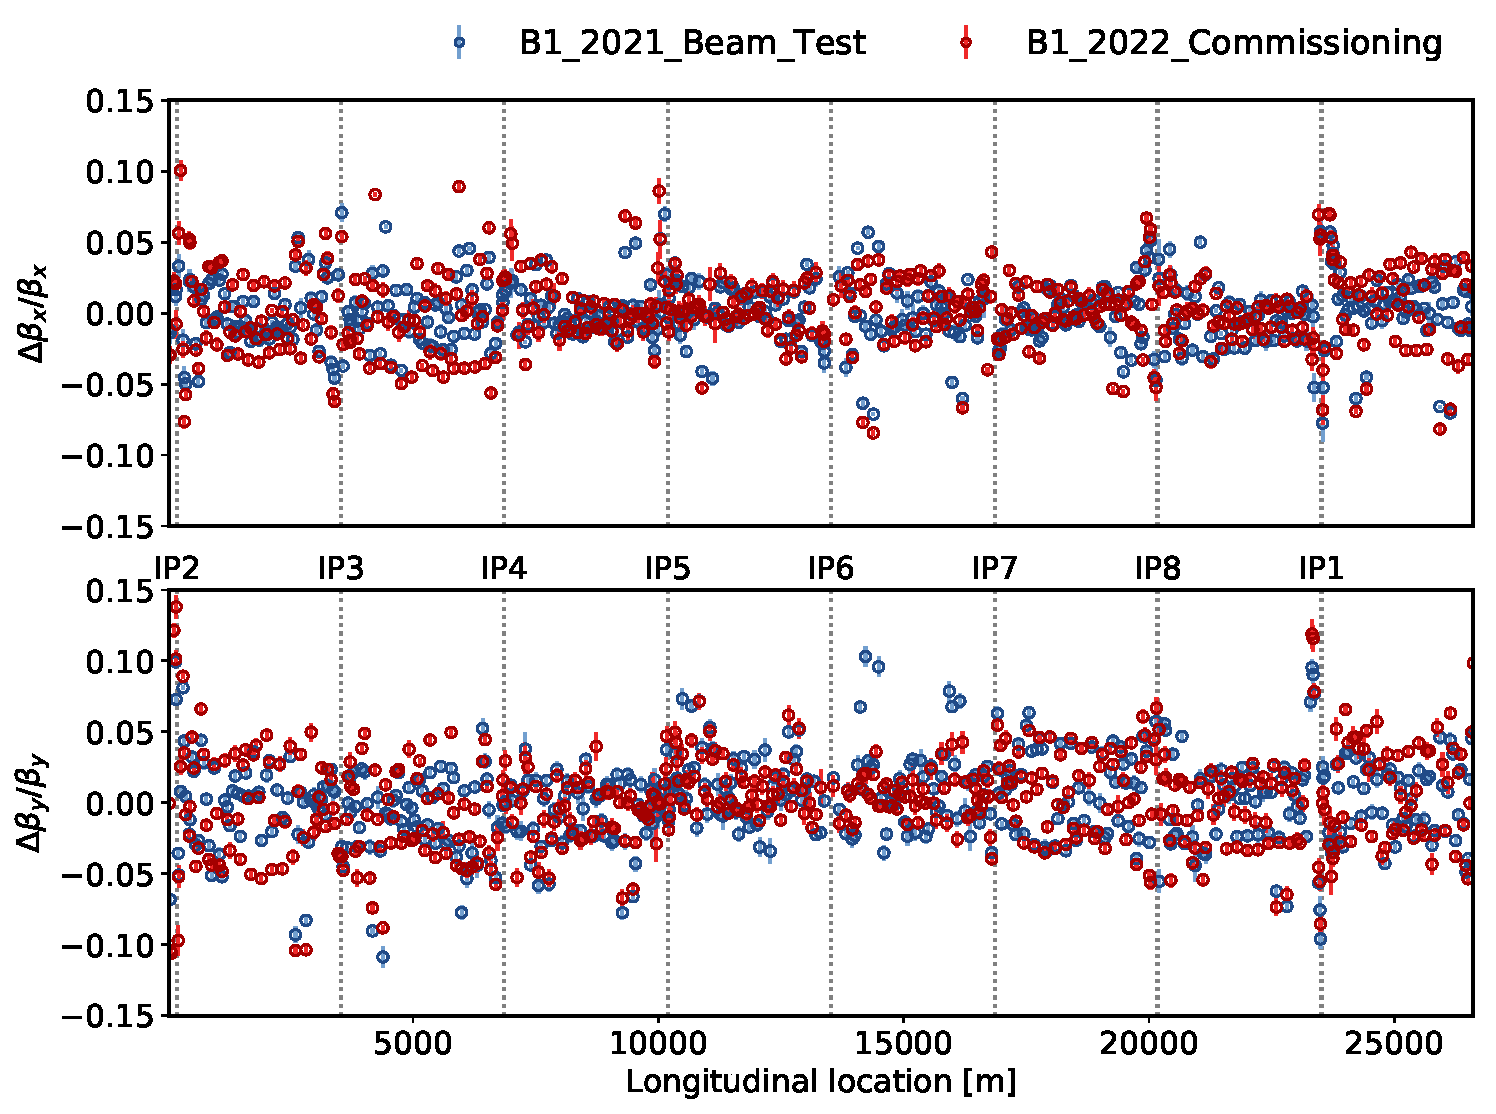
\includegraphics[width=.8\linewidth]{plots/beam1/lhcb1_betabeat_vs_beamtest.pdf}  
  \caption{Beam~1}
\end{subfigure}
\begin{subfigure}{.5\textwidth}
  \centering
  % include second image
  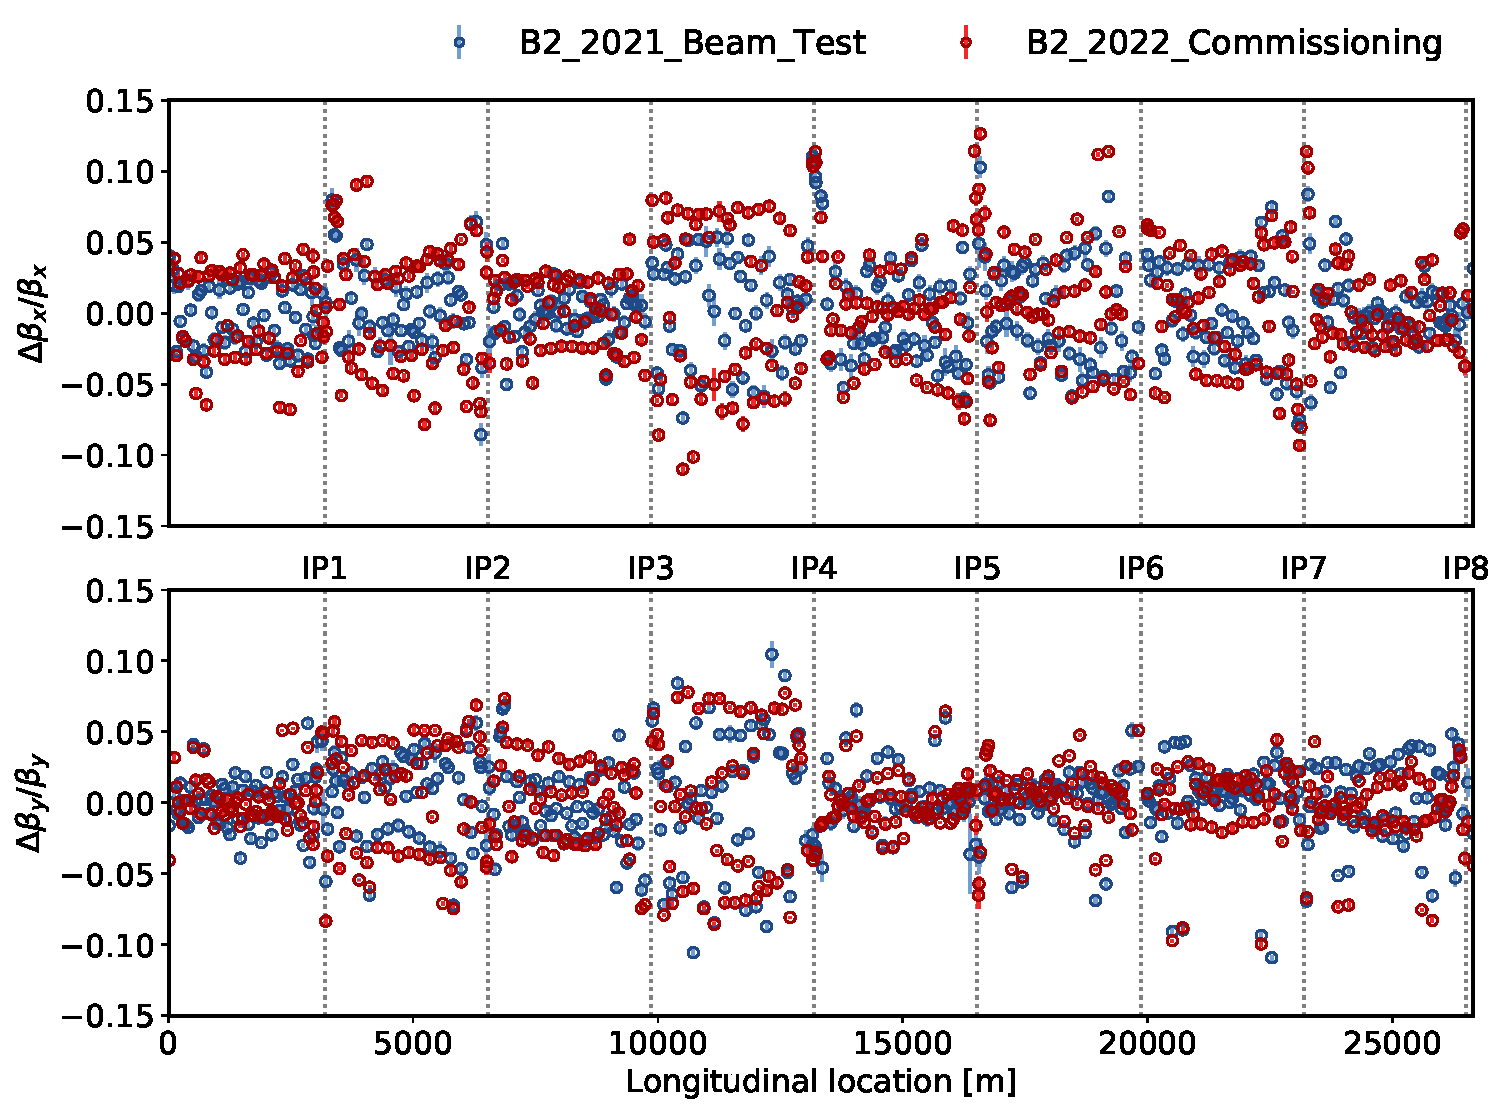
\includegraphics[width=.8\linewidth]{plots/beam2/lhcb2_betabeat_vs_beamtest.pdf}  
  \caption{Beam~2}
\end{subfigure}
\caption{The $\beta$-beating measured during the beam-test compared to what was measured in the beginning of the commissioning in 2022.}
\label{fig:2021_beta_beat_vs_2022}
\end{figure}
In order to understand the origin of the change in $\beta$-beat additional measurements were taken parasitically when other measurements were done, for example during MD and when we were measuring the ramp measurements.  



\clearpage
\section{Q'' and Q''' measurements}

Two attempts were made during the beam-test to measure the chromaticity. The first attempt was successful while the second one only was a half scan, resulting in non exploitable data. Moreover, corrections were done for this second measurement assuming last run's values.\\
The times below are local times.

\begin{longtable}[h]{l l}
  \toprule
  \textbf{Beam Process}: & SPOOLS-6.8TeV-2021\_V1@0\_[START]\\
  \textbf{Date}: & 2021-10-22 \\
  \textbf{Start Time}: & 16:05:30\\
  \textbf{End Time}: & 16:37:00\\
  \textbf{dpp range:} & -0.0027 to +0.0017 \\
  \bottomrule
  \caption{First Measurement}
\end{longtable}

\begin{longtable}[h]{l l}
  \toprule
  \textbf{Beam Process}: & SPOOLS-6.8TeV-2021\_V1@0\_[START]\\
  \textbf{Date}: & 2021-10-31\\
  \textbf{Start Time}: & 12:16:00\\
  \textbf{End Time}: & 12:30:00 \\
  \textbf{dpp range:} & -0.0033 to +0.00\\
  \midrule
  \textbf{MCO Strengths}: & B1/B2: +3.9 / +2.7 \\
  \textbf{MCD Strengths}: & B1/B2: +2316 / +2053 \\
  \bottomrule
  \caption{Second Measurement}
\end{longtable}

% Plots for Beam 1, first axis X, then Y
\begin{figure}[H]
  \centering
  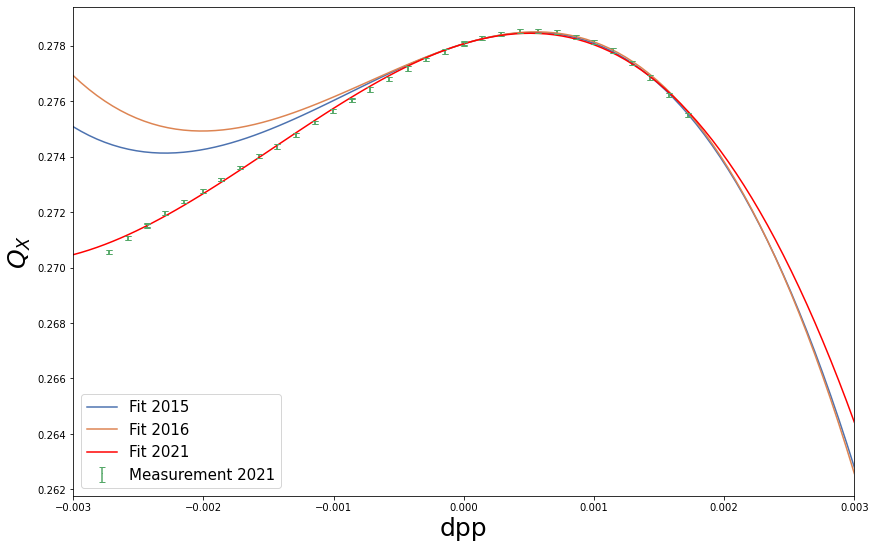
\includegraphics[width=.8\linewidth]{plots/beam1/qxb1.png}  
  \caption{Chromaticity on the X axis for Beam 1}
\end{figure}
\begin{figure}[H]
  \centering
  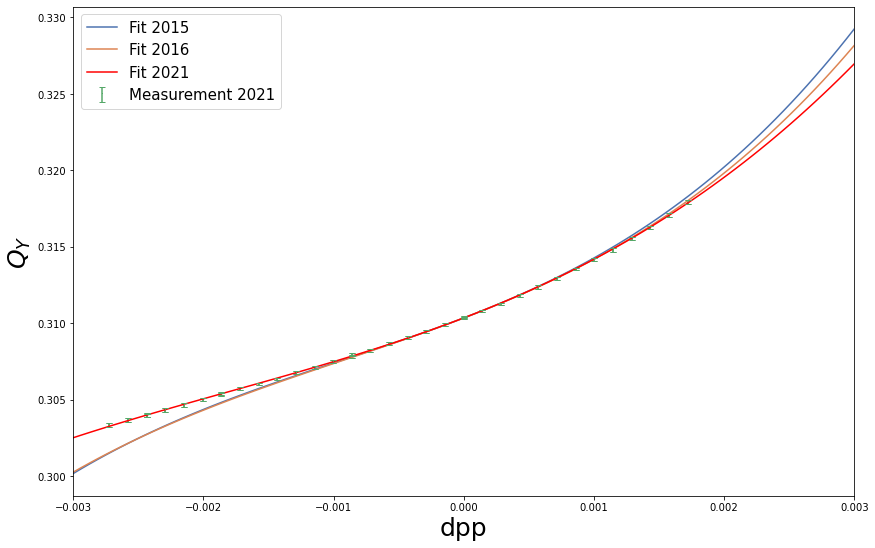
\includegraphics[width=.8\linewidth]{plots/beam1/qyb1.png}  
  \caption{Chromaticity on the Y axis for Beam 1}
\end{figure}

% Plots for Beam 2, first axis X, then Y
\begin{figure}[H]
  \centering
  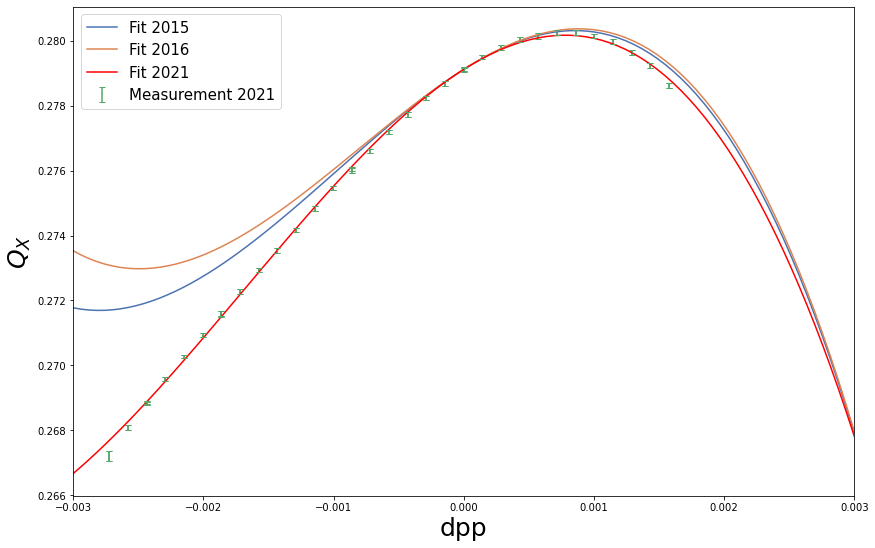
\includegraphics[width=.8\linewidth]{plots/beam2/qxb2.png}  
  \caption{Chromaticity on the X axis for Beam 2}
\end{figure}
\begin{figure}[H]
  \centering
  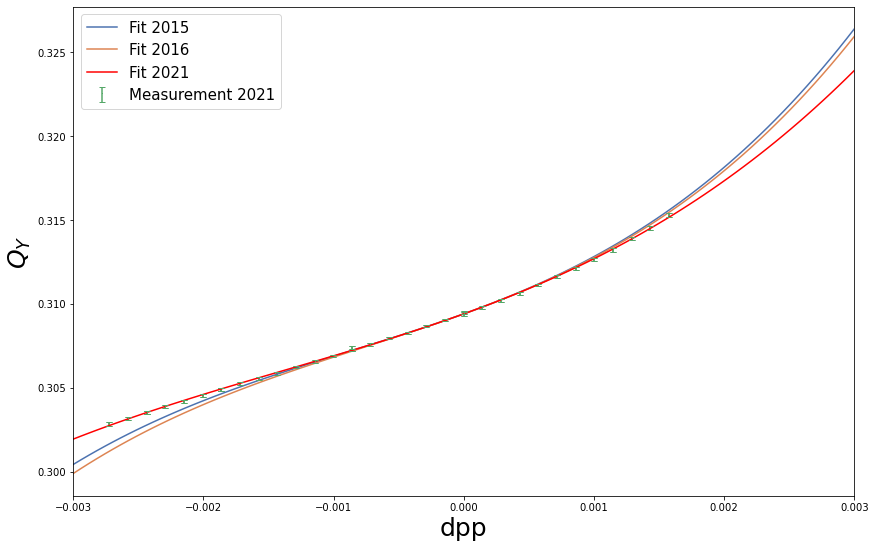
\includegraphics[width=.8\linewidth]{plots/beam2/qyb2.png}  
  \caption{Chromaticity on the Y axis for Beam 2}
\end{figure}

\begin{longtable}[h]{@{}l|c|rr|rr@{}}
  \toprule
  Year & Beam & $Q_x''[10^3]$ &   $Q_x'''[10^6]$ &   $Q_y''[10^3]$ &  $Q_y'''[10^6]$ \\
  \midrule
  \endhead
  2011 &   B1 &   $-1.8 \pm 0.03$ &  $-2.2 \pm 0.1$ &   $0.86 \pm 0.02$ &   $0.73 \pm 0.07$ \\
       &   B2 &   $-1.7 \pm 0.05$ &  $-1.1 \pm 0.1$ &   $0.82 \pm 0.02$ &   $0.90 \pm 0.06$ \\
  \midrule
  2015 &   B1 &   $-2.03 \pm 0.02$ &  $-2.31 \pm 0.08$ &   $0.97 \pm 0.02$ &   $1.06 \pm 0.04$ \\
       &   B2 &   $-2.06 \pm 0.02$ &  $-2.12 \pm 0.05$ &   $0.89 \pm 0.01$ &   $1.02 \pm 0.02$ \\
  \midrule
  2016 &   B1 &   $-1.85 \pm 0.03$ &  $-2.54 \pm 0.07$ &   $0.86 \pm 0.01$ &   $0.93 \pm 0.04$ \\
       &   B2 &   $-1.86 \pm 0.02$ &  $-2.31 \pm 0.05$ &   $0.78 \pm 0.01$ &   $1.03 \pm 0.05$ \\
  \midrule
  2021 &   B1 &   $-2.36 \pm 0.03$ &  $-1.62 \pm 0.04$ &  $0.98 \pm 0.01$ &  $0.55 \pm 0.02$ \\
       &   B2 &   $-2.64 \pm 0.03$ &  $-1.56 \pm 0.05$ &  $0.78 \pm 0.01$ &   $0.58 \pm 0.02$ \\
  \bottomrule
  \caption{Non Linear Chromaticity Results and History}
\end{longtable}


\section{MCS feed-down}
It has been observed that changing the strength of the MCS ($b_3$ spool pieces) have an impact on the transverse coupling in the LHC. The main hypothesis is that this is coming from a vertical misalignment of the MCS or from a systematic orbit effect. In order to validate if the effect had remained constraint after the Long Shutdowns a new measurement was carried out during the beam-test. The result for Beam~1 is show in in Fig.~\ref{fig:beam1_mcs} and for Beam~2 in  Fig.~\ref{fig:beam2_mcs}. Beam~1 has less measurements since the MD in 2018 was only for Beam~2. We observe that both the amplitude and the sign seems to have stayed constant between Run~2 and Run~2. This is an important observation since this indicates that the coupling feed-down caused by this could be mitigated as proposed in YYY. In fact the proposal to compensate the dynamic part of the b3-decay was implemented in 2022 a final analysis of the impact of this will be reported later.

\begin{figure}[ht]
\begin{subfigure}{.5\textwidth}
  \centering
  % include first image
  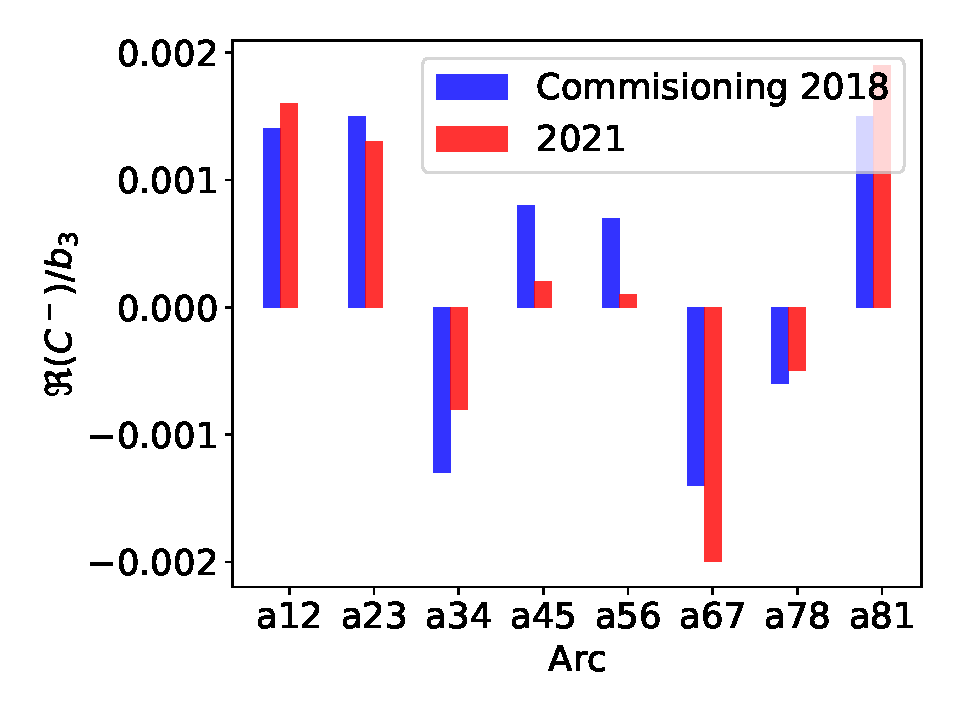
\includegraphics[width=.8\linewidth]{plots/MCS/b_1change_re_per_b3.pdf}  
  \caption{Real part of the $C^-$.}
\end{subfigure}
\begin{subfigure}{.5\textwidth}
  \centering
  % include second image
  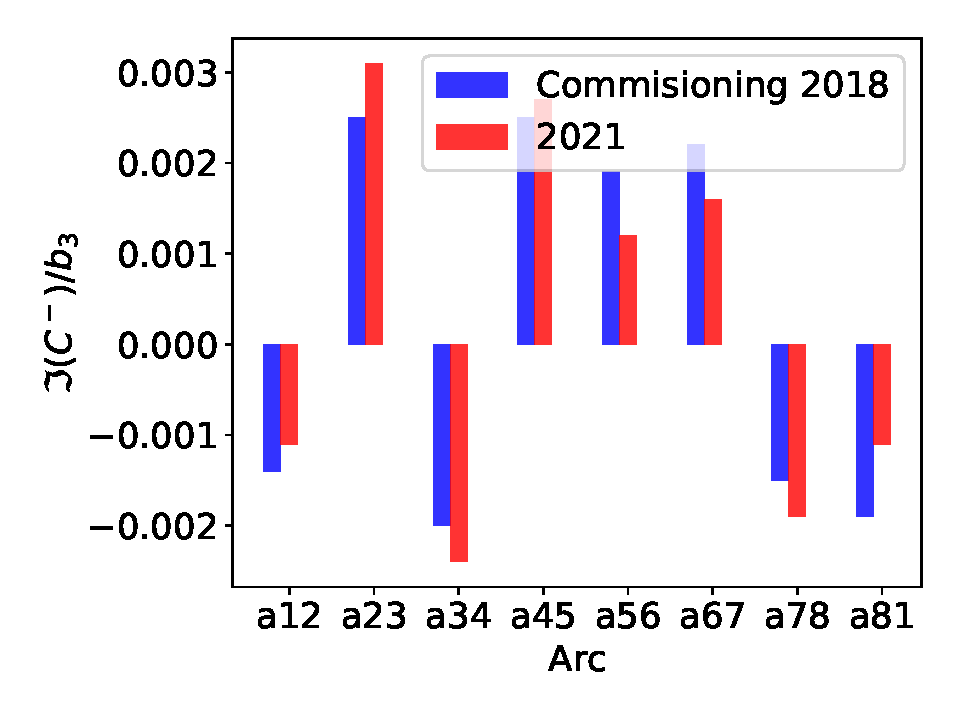
\includegraphics[width=.8\linewidth]{plots/MCS/b_1change_im_per_b3.pdf}  
  \caption{Imaginary part of the $C^-$.}
\end{subfigure}
\caption{The impact on the $C^-$ from changing the MCS corrector ($b_3$-spool pieces) for Beam~1. }
\label{fig:beam1_mcs}
\end{figure}

\begin{figure}[ht]
\begin{subfigure}{.5\textwidth}
  \centering
  % include first image
  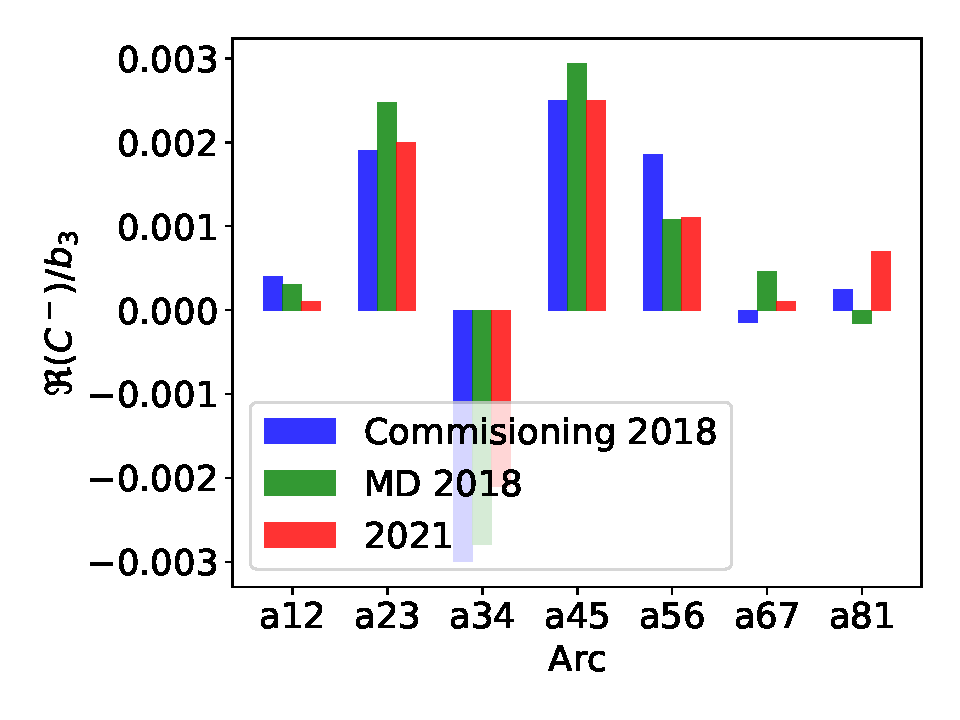
\includegraphics[width=.8\linewidth]{plots/MCS/b2_change_re_per_b3.pdf}  
  \caption{Real part of the $C^-$.}
\end{subfigure}
\begin{subfigure}{.5\textwidth}
  \centering
  % include second image
  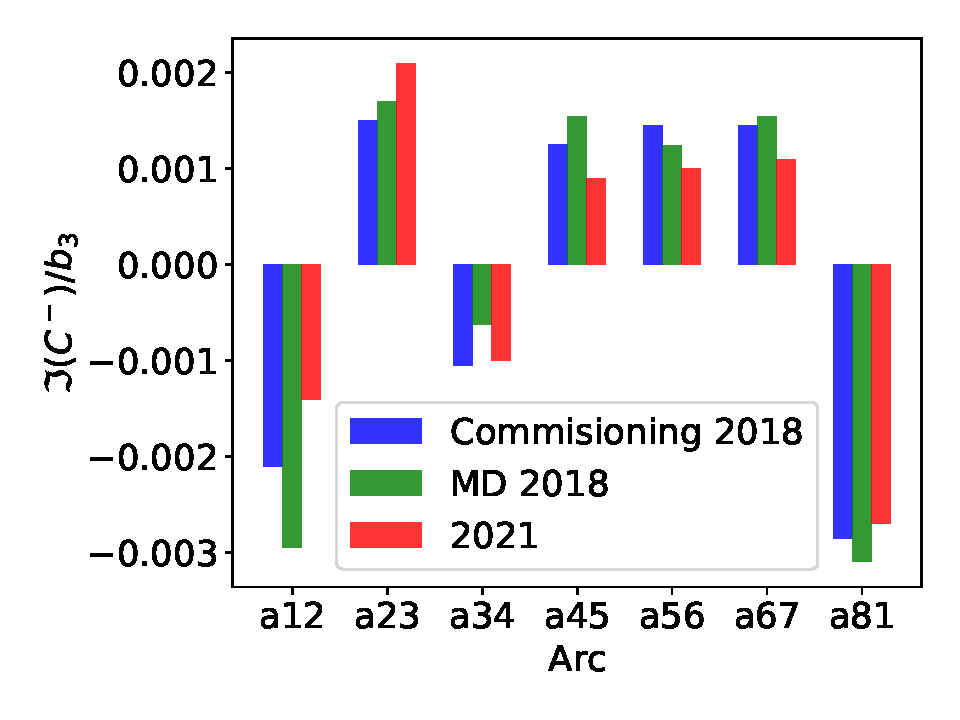
\includegraphics[width=.8\linewidth]{plots/MCS/b_2change_im_per_b3.pdf}  
  \caption{Imaginary part of the $C^-$.}
\end{subfigure}
\caption{The impact on the $C^-$ from changing the MCS corrector ($b_3$-spool pieces) for Beam~1.}
\label{fig:beam2_mcs}
\end{figure}


\section{Summary and Outlook}
The optics corrections during the beam test was very successful in terms of demonstrating the readiness of the optics corrections tools as well as finding the swap of the magnet RRR. Furthermore, it was very useful in testing the tools and software packages to be ready for Run~3. The optics corrections also remained the same for the 2023 Run. A degradation of the optics quality was observed for Beam~2 but not for Beam~1. Through simulations it has been excluded to derive from energy variations at injection. Instead it is more likely that it dervies from hysteresis or/and decays at injection. It would be interesting to measure the optics at different intervals over a longer time period. This could potentially be combined with a scrubbing run where one could apply kicks between the fills for scrubbing. 

\begin{thebibliography}{99}   % Use for  1-9  reference

\bibitem{ats_stephane}
S.~Fartoukh, ``Achromatic telescopic squeezing scheme and its application to the LHC and its luminosity upgrade'', Phys. Rev. ST Accel. Beams {\bf16}, 111002 (2013)

\bibitem{roderik} R. Bruce, {\it et al.}, ``New IR7 optics with removed
MQW magnets'',  \href{https://indico.cern.ch/event/681507/contributions/2814548/attachments/1570845/2478033/2017.12.06--HSS_meeting_MQW_removal.pdf}{ABP-HSS Section meetings
Wednesday 6 Dec. 2017}.

\bibitem{run3} S. Fartoukh, {\it et al.}, 
	``LHC Configuration and Operational Scenario for Run 3'', CERN-ACC-2021-0007.

\bibitem{ACcom} T.~Persson, {\it et al.}, ``LHC optics commissioning: A journey towards 1$\%$ optics control'', Phys. Rev. Accel. Beams, \textbf{20}, 061002 (2017).
\url{https://doi.org/10.1103/PhysRevAccelBeams.20.061002}

\bibitem{ewen2019jour} E.H. Maclean, {\it et al.}, ``A new approach to the LHC optics commissioning for the nonlinear era'', {\it Phys. Rev. Accel. Beams}  {\bf 22}, p. 061004 (2019).\vspace{-0.03cm}
\url{https://doi.org/10.1103/PhysRevAccelBeams.22.061004}


	


\bibitem{first} M. Aiba, S. Fartoukh, A. Franchi, M. Giovannozzi, V. Kain, M. Lamont, R. Tom\'as, G. Vanbavinckhove, J. Wenninger, F. Zimmermann, R. Calaga, and A. Morita, ``First beta-beating measurement and optics analysis for the CERN Large Had ron Collider'', Phys. Rev. ST Accel. Beams {\bf12}, 081002 (2009).

\bibitem{michiEvian} M. Hostettler, ``The 2021 beam test results & lessons learned'', Evian OP Workshop 2021, CERN, Switzerland. 
\url{https://indico.cern.ch/event/1077835/contributions/4533367/attachments/2350863/4009681/2021_Evian_BeamTest.pdf}


\bibitem{tomasCERNLargeHadron2010}
R. Tomás, {\it et al.}, “CERN Large Hadron Collider optics
model, measurements, and corrections”, {\it Phys. Rev. Accel. Beams}  {\bf 13}, p. 121004 (2010).
%
\bibitem{record} R. Tom\'as, {\it et al.}, ``Record low beta beating in the LHC'',
Phys. Rev. ST Accel. Beams {\bf15}, 091001, 2012.
%
\bibitem{felixkmod} F. Carlier and R. Tom\'as, ``Accuracy and feasibility of the $\beta^*$ measurement for LHC and High Luminosity LHC using k-modulation'',
Phys. Rev. Accel. Beams {\bf20}, 011005 (2017).
%

%https://journals.aps.org/prab/pdf/10.1103/PhysRevSTAB.13.121004

\bibitem{jaime_rdt}
J. Coello, R. Tom\'as and M. Hofer, ``New local optics measurements and correction techniques for the LHC and its luminosity upgrade'', Phys. Rev. Accel. Beams {\bf 23}, 041001 (2020).
\url{https://doi.org/10.1103/PhysRevAccelBeams.23.041001}

\bibitem{cardona17} J. F.  Cardona, A. C. Garc\'ia, and R. Tom\'as, ``Local correction of quadrupole errors at LHC interaction regions using action and phase jump analysis on turn-by-turn beam position data'', {\it Phys. Rev. Accel. Beams} {\bf 20}, p. 111004 (2017).
\url{https://doi.org/10.1103/PhysRevAccelBeams.20.111004}

\bibitem{cardona20} J. F.  Cardona, Y. Rodr\'iguez, and R. Tom\'as, ``A twelve-quadrupole correction for the interaction regions of high-energy accelerators'',  arXiv:2002.05836 [physics.acc-ph] (2020).

%\cite{Garcia Morales:IPAC21-MOPAB186}
\bibitem{Garcia_Morales:IPAC21-MOPAB186}
   H. Garcia Morales, {\it et al.},
   \textquotedblleft{Comparison of Segment-by-Segment and Action-Phase-Jump Techniques in the Calculation of IR Local Corrections in LHC}\textquotedblright,
   in \emph{Proc. IPAC’21}, Campinas, Brazil, May 2021, pp. 632--635.
   \url{doi:10.18429/JACoW-IPAC2021-MOPAB186}  

\bibitem{ipac2022_apj} J. F. Cardona, {\it et al.}, ``Progress on the action and phase jump for LHC local optics correction'', this conference.


\bibitem{IPAC2020Fol}  E. Fol, {\it et al.},
   \textquotedblleft{Machine Learning Techniques for Optics Measurements and Corrections}\textquotedblright,
   in \emph{Proc. IPAC’20}, Caen, France, May 2020, pp. 61.
   \url{doi:10.18429/JACoW-IPAC2020-WEVIR12} 

\bibitem{epj_efol} E.~Fol, R.~Tom\'as,  G.~Franchetti. ``Supervised learning-based reconstruction of magnet errors in circular accelerators'', Eur.~Phys.~J.~Plus 136, 365 (2021). \url{doi.org/10.1140/epjp/s13360-021-01348-5}

\bibitem{efol_mlcorr_this_conference} E.~Fol, {\it et al.}, ``Experimental Demonstration of Machine Learning Application in LHC Optics Commissioning'', this conference.


\bibitem{evian_2015_langer} A. Langner, {\it et al.}, “Optics model”, Proceedings of the 6th Evian Workshop,
Evian, France, (2015) \url{https://indico.cern.ch/event/434129/contributions/1917199/attachments/1223733/1790347/EVIAN_alangner.pdf}
%
\bibitem{tobias_evian19}
T.~Persson, {\it et al.}, ``LHC Optics Corrections in Run 2, LHC operation Workshop Evian Workshop 2019, Evian France.
\url{https://indico.cern.ch/event/751857/contributions/3259376/attachments/1781875/3033022/optics_corrections_run2.pdf}
%
\bibitem{felix_soubelet_local_coupling_this_conference} F.~Soubelet, {\it et al.}, ``First Interaction Region Local Coupling Corrections in the LHC Run~3'', this conference.
%
\bibitem{michaelcoup} M. Hofer and R. Tom\'as, ``Effect of local linear coupling on linear and nonlinear observables in circular accelerators'',
Phys. Rev. Accel. Beams {\bf23}, 094001, 2020.
%
\bibitem{MDlocalcoupling} T.~Persson, {\it et al.}, ``MD4944: Local linear coupling measurement at the IPs'', CERN-ACC-NOTE-2020-0013.

%\cite{Soubelet:IPAC21-MOPAB007}
\bibitem{Soubelet:IPAC21-MOPAB007}
   F. Soubelet,  {\it et al.} ,
   \textquotedblleft{Prospect for Interaction Region Local Coupling Correction in the LHC Run 3}\textquotedblright,
   in \emph{Proc. IPAC’21}, Campinas, Brazil, May 2021, pp. 61--64.
   \url{doi:10.18429/JACoW-IPAC2021-MOPAB007}  

\bibitem{coup_improved_tpersson} T. Persson and R. Tom\'as, ``Improved control of the betatron coupling in the Large Hadron Collider'',
{\it Phys. Rev. ST Accel. Beams} {\bf 17}, p. 051004 (2014).
\url{https://doi.org/10.1103/PhysRevSTAB.17.051004}
%
\bibitem{ipac2018_automatic_coupling}    T. Persson \emph{et al.},
   \textquotedblleft{Transverse Coupling Measurements With High Intensity Beams Using Driven Oscillations}\textquotedblright,
   in \emph{Proc. IPAC’18}, Vancouver, Canada, Apr.-May 2018, pp. 208--211.
   \url{doi:10.18429/JACoW-IPAC2018-MOPMF047}    
%
\bibitem{josch} J. Dilly, {\it et al.}, ``Controlling Landau damping via feed-down from high-order correctors in the LHC and HL-LHC'', IPAC 2022, this conference.

\end{thebibliography}
\appendix
\section{Decay compensation}
Based on the measurement of the feed-down from the MCS to coupling a new powering to compensate for the b3 decay in the dipoles have been calculated. It is matched in such a way that it compensates the chromaticity by the same amount as the even compensation but distributed in such a way that the coupling is expected to stay constant. The knobs for this are the following:
\begin{verbatim}

RCS.A12B1/K2 0.8630127907663837 
RCS.A23B1/K2 0.779866457813889 
RCS.A34B1/K2 1.3828734821095998 
RCS.A45B1/K2 0.4445174033278492 
RCS.A56B1/K2 0.9114975331776818 
RCS.A67B1/K2 1.401218693590656 
RCS.A78B1/K2 1.3540008484475567 
RCS.A81B1/K2 0.8630127907663839 

RCS.A12B2/K2 0.6866554457561092 
RCS.A23B2/K2 0.9619053275562472 
RCS.A34B2/K2 1.5867931783979445 
RCS.A45B2/K2 0.7923501971731068 
RCS.A56B2/K2 0.9643136781336532 
RCS.A67B2/K2 1.391600462298758 
RCS.A78B2/K2 1.16296351210475 
RCS.A81B2/K2 0.5945946691676663 

\end{verbatim}
\end{document}
